% !TEX root = ../my-thesis.tex
%
\chapter{Place du rehaussement dans l'analyse d'images}

% TODO : S'assurer que les différentes catégories scientifiques sont là
% TODO : Vérifier qu'il y a bien une justification vers un choix de progression et des parties dé-corélées sans fil conducteur.

\cleanchapterquote{Un petit chapitre pour le doctorant, un grand chapitre pour l'humanité}{Doctorant anonyme}{(Citation temporaire)}

\section{Problématiques}
    \subsection{Visualisation}

    Nous avons abordé dans le chapitre précédent les deux méthodes d'acquisitions utilisées par l'imagerie du foie en exposant leurs avantages et leurs limites. Nous avons aussi présenté les différentes bases de données publiques disponibles et discuté de leur potentiel en tant que bases d'évaluation d'algorithmes.

    Bien que nous ayons montré de nombreuses illustrations dans le chapitre précédent, nous n'avons pas abordé la manière de visualiser ces données.
    Le problème initial des médecins est en effet de détecter visuellement des anomalies liées à des pathologies dans ces images. Après les étapes d'acquisition et de reconstruction, les images sont présentées selon deux formes similaires : Un ensemble d'images 2D correspondant aux coupes d'acquisition ou un volume 3D, d'un seul bloc, contenant la superposition des coupes.
    
    La première méthode d'analyse, encore beaucoup utilisée par les médecins aujourd'hui est la visualisation des coupes 2D des organes (Fig. \ref{fig:slice_visualization}). De la même manière que la TDM ou l'IRM, le médecin visualise l'image coupe par coupe. Cette visualisation nécessite cependant de l'entrainement et une réelle connaissance des organes étudiés, car le médecin doit reconstituer mentalement le volume des structures observées à partir des images 2D. Cette méthode a toutefois l'avantage de ne nécessiter presque aucun traitement (à part un ajustement dynamique des contrastes) et permet de visualiser l'ensemble de l'image sans problèmes de recouvrement ou d'obstruction entre les structures. 

    \begin{figure}[!ht]
      \centering
      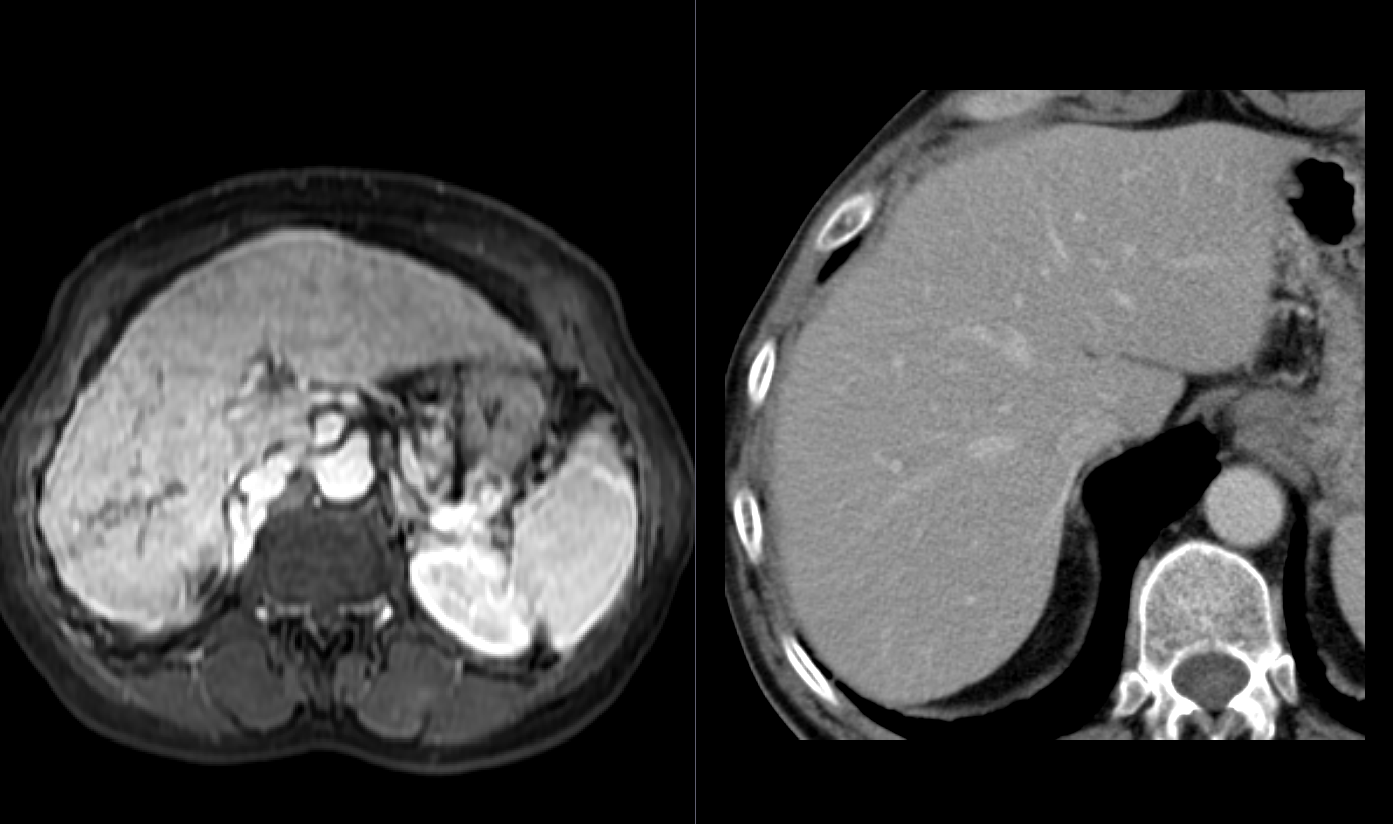
\includegraphics[height=5cm]{Images/2D_view.png}
      \caption{La visualisation en coupe est la méthode la plus utilisée par les médecins. Celle-ci nécessite toutefois de se représenter mentalement la structure 3D de l'organe. À gauche IRM, à droite tomodensitométrie.}
      \label{fig:slice_visualization}
    \end{figure}

    La visualisation 3D, où l'on travaille avec le volume 3D, facilite cet exercice. Elle permet en effet de visualiser directement les structures dans leur entièreté. Cependant, elle nécessite d'une manière ou d'une autre de hiérarchiser l'information brute de l'image. Dans le cas contraire, l'information nécessaire au diagnostique reste cachée (\ref{fig:hierachy_3D}). On peut distinguer deux méthodes pour résoudre ce problème : La première consiste à hiérarchiser les données par projection alors que la seconde identifie et extrait les structures d'intérêt.
    
    \begin{figure}[!ht]
      \centering
      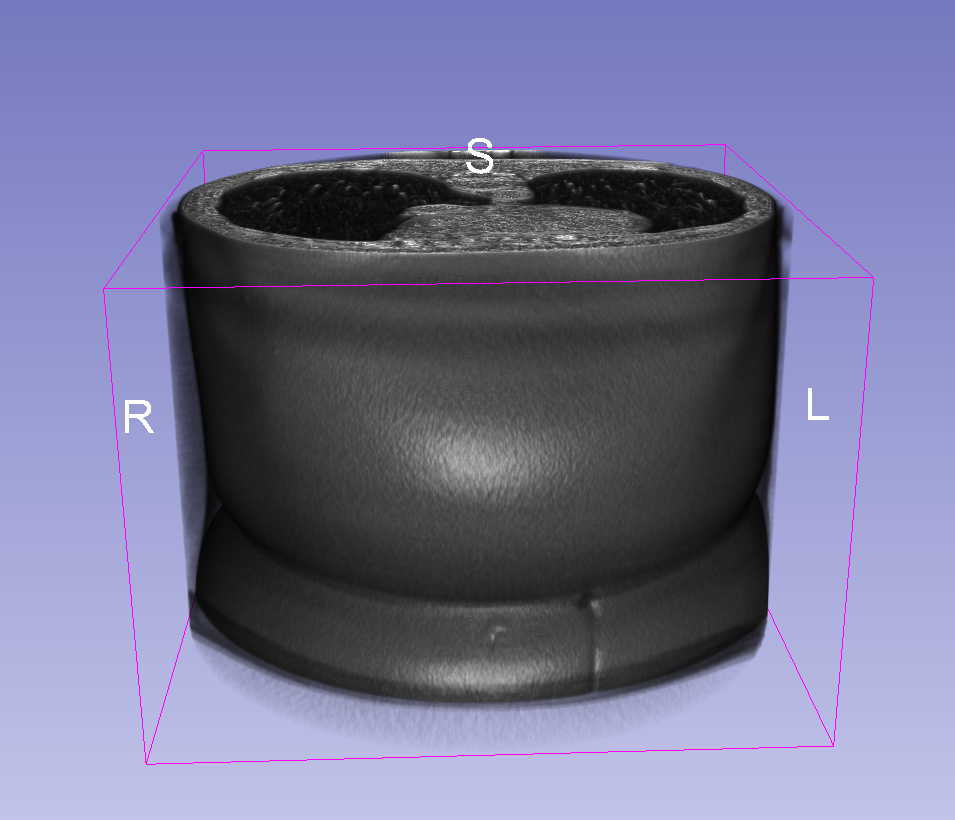
\includegraphics[height=5cm]{Images/hierarchy_3D.png}
      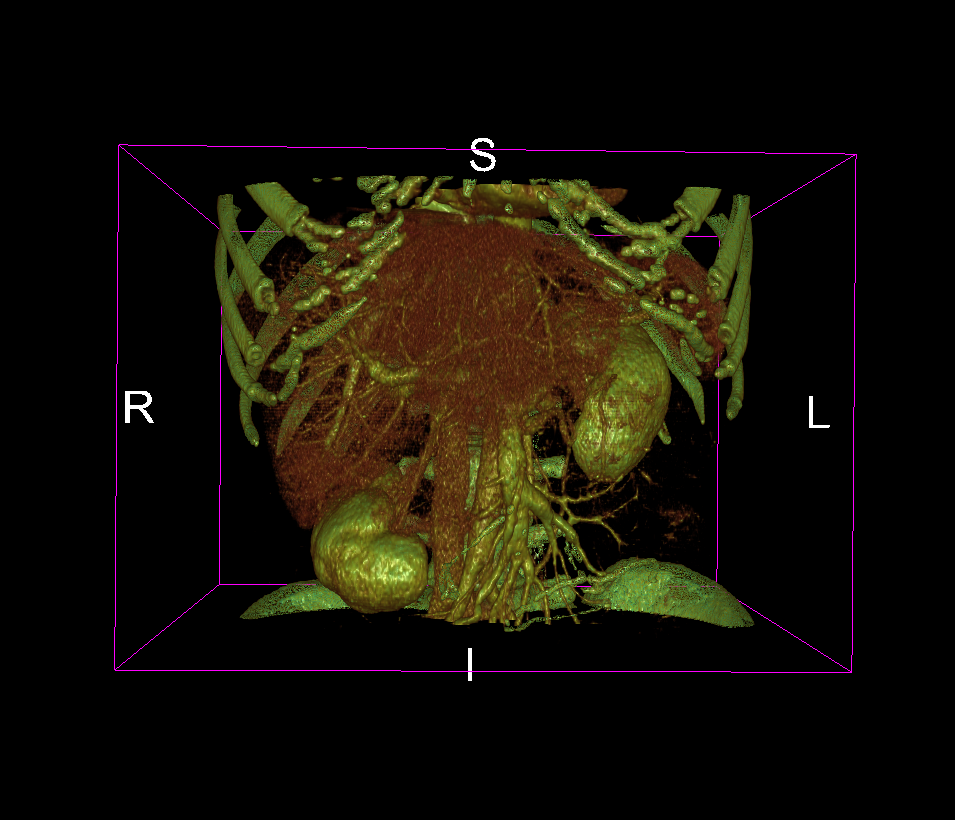
\includegraphics[height=5cm]{Images/hierarchy_3D_bis.png}
      \caption{Rendu surfacique d'un volume 3D. Sans hiérarchisation de l'information, les structures d'intérêt restent cachées. En hiérarchisant l'information (seuils d'opacité et de couleurs en fonction de l'intensité des voxels), on peut observer les structures anatomiques d'intérêts. Un traitement naïf ne suffit toutefois pas à différencier toutes les structures.}
      \label{fig:hierachy_3D}
    \end{figure}


      \subsubsection{Maximum Intensity Projection}
      La MIP (Maximum Intensity Projection) est une technique de projection permettant de visualiser les éléments les plus saillants d'une image. En pratique, elle consiste à créer un plan image 2D $P$ puis pour chaque pixel $p_i$ de ce plan à lancer un rayon qui traverse le volume 3D. Pour l'ensemble des voxels qui intersectent le rayon, on récupère la valeur maximale parmi leur intensité que l'on affecte à $p_i$ (Fig. \ref{fig:MIP_visualisation}). 

      \begin{figure}[h]
        \centering
        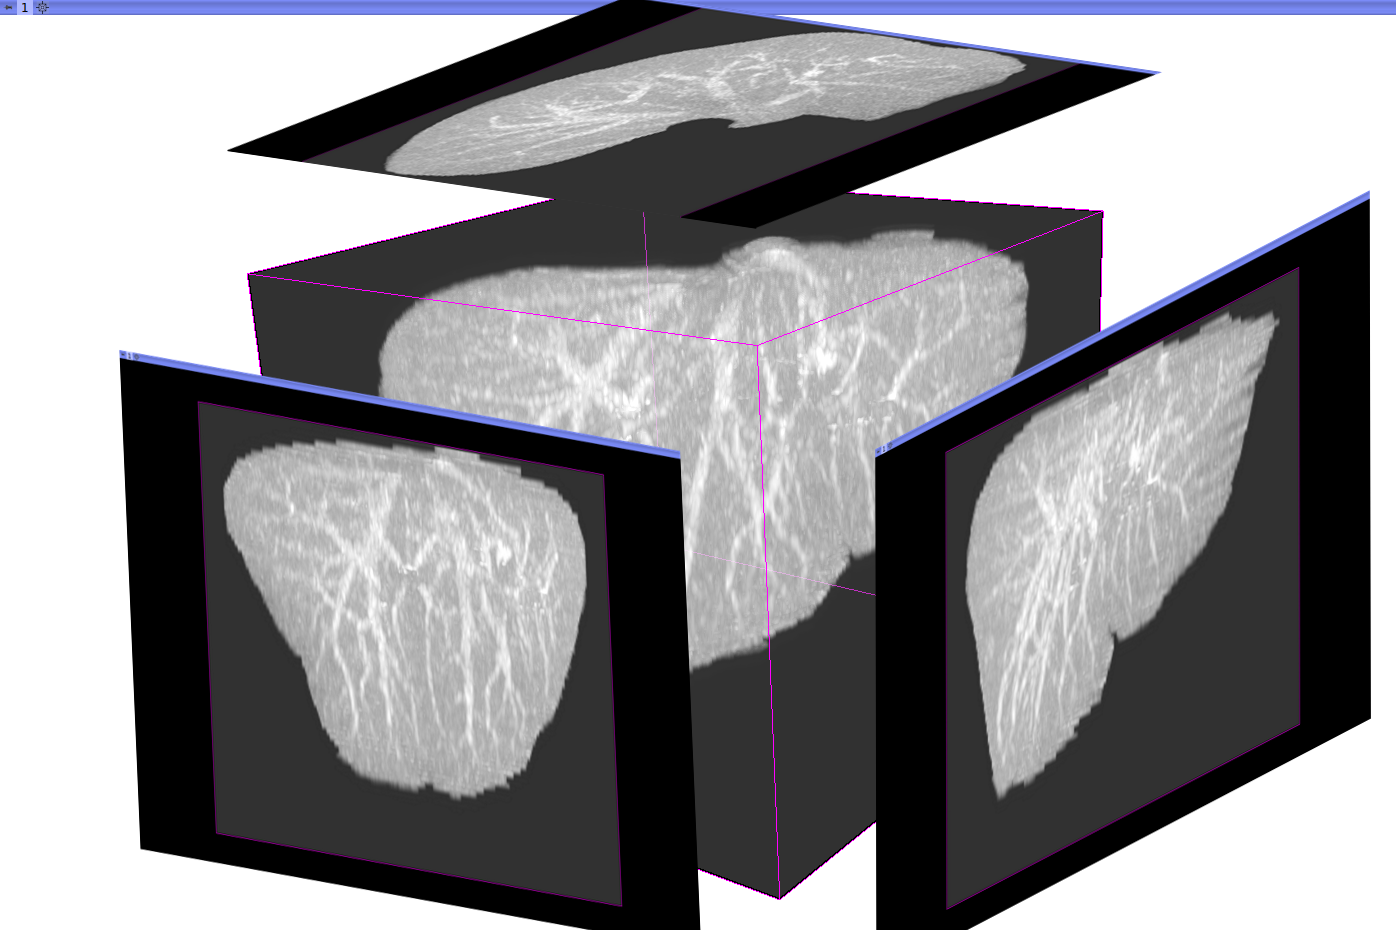
\includegraphics[height=5cm]{Images/3D_mip_montage.png}
        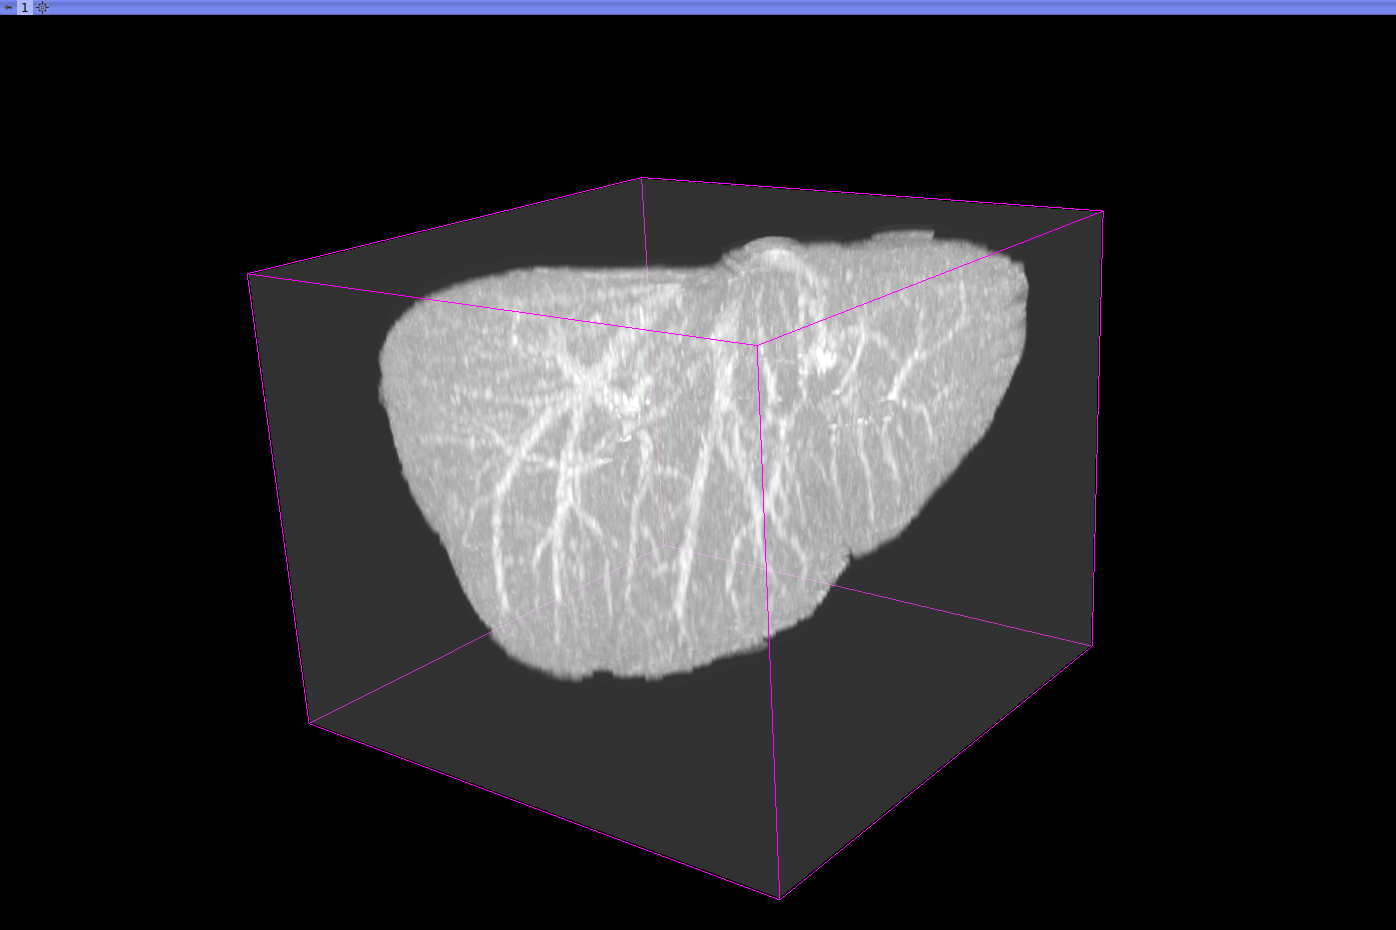
\includegraphics[height=5cm]{Images/3D_mip.png}
        \caption{Maximaly intensity projection. L'intensité maximale est projetée le long du rayon sur le plan d'origine. La MIP peut s'effectuer en utilisant les bords de l'image, où le plan de la caméra dans une scène 3D}
        \label{fig:MIP_visualisation}
      \end{figure}

      Cette méthode permet de faire ressortir les éléments les plus intenses de l'image et convient particulièrement à des structures mises en valeur par agent de contraste. Elle est simple à implémenter et peu coûteuse en calcul. Elle fait cependant perdre toute perception de profondeur par la projection des maxima sur le plan image. 
      
      Par exemple, une MIP dont les rayons sont lancés du plan antérieur vers le plan postérieur produit la même image (à effet miroir prêt) qu'une MIP dont les rayons sont lancées du plan postérieur vers le plan antérieur.

      La perte de profondeur se compense lorsque dans une scène 3D, le plan de projection devient le plan de la caméra. Le mouvement de la caméra permet alors de résoudre les ambiguïtés provoquées par un seul plan de projection en simulant, dans une certaine mesure, la stéréoscopie de la vision humaine.
      La MIP a aussi le désavantage d'être parasitée par toutes structures plus intenses que l'organe observé. L'observation du foie et de ses vaisseaux en MIP est notamment perturbée par les os de la cage thoracique. Ce problème peut cependant être contourné en appliquant un masque pour ne conserver que le foie, ce qui demande un coût supplémentaire d'annotation.

      \subsubsection{Segmentation}
      
      D'autres moyens de visualisation sont possibles, par exemple en représentant un modèle 3D des structures observées. On peut ainsi visualiser des organes seuls, sans éléments adjacents perturbateurs (Fig. \ref{fig:segmentation_3D}). La création de ce modèle nécessite un traitement plus complexe des données afin d'identifier, de classer, de filtrer puis d'extraire les structures d'intérêt. C'est ce processus que l'on nomme la segmentation. La segmentation automatique reste un domaine de recherche ouvert, car les nombreux artefacts de la TDM et de l'IRM complexifie fortement la problématique.
      
      Là où l'utilisation de la MIP est limitée dans ses usages, la segmentation est utilisée non seulement pour la visualisation, mais aussi pour des applications plus larges comme la simulation ou le calcul du volume d'un réseau vasculaire où une plus grande précision est demandée.
      
      Dans la suite de ce chapitre, nous présentons les grandes familles d'algorithmes de segmentation avant d'introduire les filtres de rehaussement de vaisseaux qui sont au cœur de nos travaux.

      \begin{figure}[h]
        \centering
        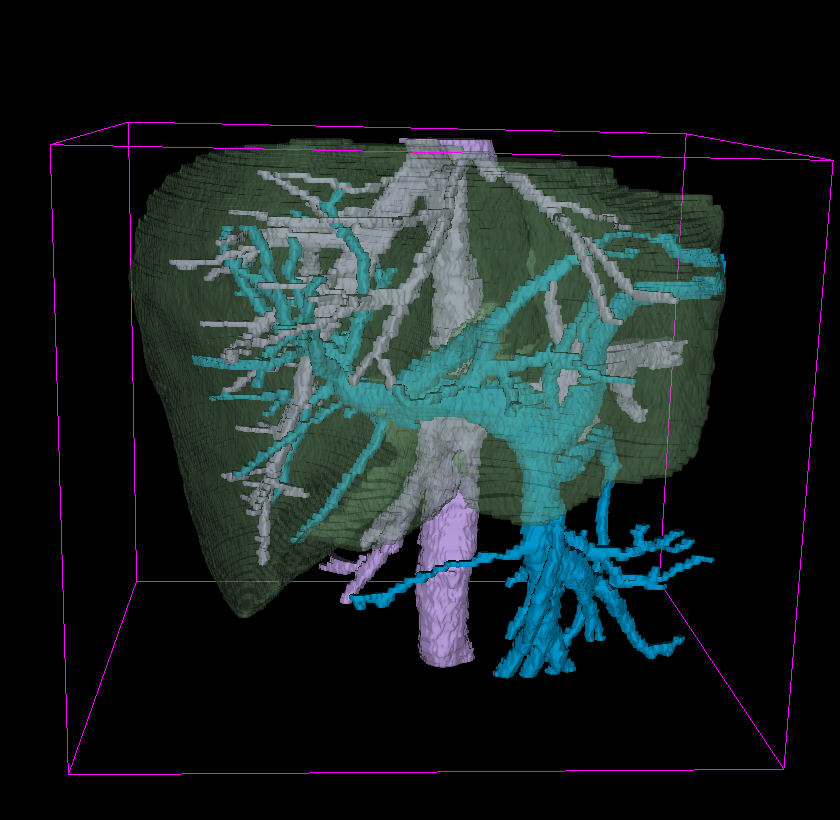
\includegraphics[height=5cm]{Images/segmentation_3D.png}
        \caption{Segmentation du foie (vert) et des deux réseaux vasculaires hépatiques (veine porte en bleu et veine cave en violet).}
        \label{fig:segmentation_3D}
      \end{figure}
  
  \subsection{Extraction de structures d'intérêts}

      Parmi la littérature sur l'extraction de structures d'intérêts, deux sujets sont fortement liés : l'amélioration de la qualité des images et les algorithmes de segmentation.

    \subsubsection{Amélioration du signal}
      
    Historiquement, le besoin d'améliorer la qualité des images provient des limitations des premières machines d'imagerie. Il était alors nécessaire de développer des méthodes efficaces pour limiter les artefacts tel que le bruit et ainsi faire ressortir les organes d'intérêt. 
    
    De nombreuses méthodes ont cherché à caractériser, estimer puis corriger le bruit. Gudbjartsson et al. \cite{Gudbjartsson1995r_Rician_noise_MRI} ont explicité le caractère ricien du bruit en IRM. Dietrich et al. proposent une validation des approches pour calculer le SNR en fonctions des différentes méthodes d'acquisition et de la reconstruction des images IRM. Gravel et al. \cite{Gravel_2004_estimate_noise_medical_img} propose une méthode capable d'estimer la nature du bruit en fonction de sa variance et de l'intensité de l'image. Enfin, Krissian et al. \cite{Krissian_2009_diffusion_MRI}et Mendrik et al. \cite{Mendrik2009_HDCS} cherchent à lisser le bruit par un mécanisme de diffusion. Le premier, propose d'estimer automatiquement le bruit grâce à sa variance pour paramétrer le lissage. Le second propose un lissage adaptatif continu permettant de s'adapter à la géométrie locale.    
    
    De nos jours, les progrès techniques et l'amélioration de la résolution des machines ont résolu beaucoup de ces problèmes. La recherche de gains de performances se tourne de plus en plus vers de l'apprentissage qui permet d'améliorer à la fois la qualité des images et d'accélérer les traitements existants. C'est par exemple le cas de méthodes à base de deep learning \cite{Higaki2019_deep_MRI_CT_quality} qui permettent d'améliorer la résolution et de corriger le bruit.

    L'amélioration globale du signal a un effet positif sur les structures anatomiques qui présentent une intensité localement plus homogène ainsi que des contours mieux définis. Leur extraction par des algorithmes de segmentation en est donc facilitée.

    \subsubsection{Extraction}

      Les algorithmes d'extractions en imagerie médicale sons les mêmes que l'on retrouve pour des images issues de la photographie classique. La plupart sont sous la forme d'un problème d'optimisation dans lequel on définit une énergie à minimiser.

      \paragraph{Courbes de niveaux} 
      Les courbes de niveaux sont des méthodes qui font s'étendre un contour en fonction du temps, jusqu'à ce qu'un critère d'arrêt soit atteint. Ce critère peut reposer sur un modèle des structures à segmenter, des caractéristiques de l'image ou des propriétés sur la courbure du front de propagation du contour.

      La méthode développée par Kass et al. \cite{Kass1988_snakes} (aussi appelés \textit{snakes}) est l'une des méthodes de contours actifs les plus populaires. 
      
      Cette méthode formule l'énergie contrôlant la propagation du contour comme la somme pondérée d'une énergie interne et d'une énergie externe que l'algorithme cherche à minimiser. L'énergie interne est liée au modèle et contraint l'expansion (par exemple une énergie liée à un modèle géométrique) alors que l'énergie externe (basé par exemple sur les gradients de l'image) favorise la propagation du contour. Cette énergie a ensuite connue de nombreuses variations comme Wang et al. \cite{Wang2012_vessel_level_set} qui proposent un modèle minimisant trois énergies : une énergie basée sur la courbure du contour, une énergie basée sur les gradients d'intensités de l'image et une énergie basée la correspondance du contour à un modèle cylindrique. Zeng \cite{Zeng2018_liver_hybrid_active_contour_region_growing} utilise les contours actifs pour segmenter les gros vaisseaux, sans débordement des structures. La paramétrisation du contour actif est basé sur l'estimation de l'intensité des vaisseaux fins détectés par un filtre bi-gaussien.

      L'utilisation des contours actifs sous cette forme est particulièrement efficace sur des objets relativement convexes. Lorsque la géométrie des structures est plus complexe ou très alongée, la propagation du contour est plus difficile. De plus, l'implémentation du suivi des contours est difficile lorsque des changements de topologie ont lieux. C'est le cas, par exemple, de la séparation du contour en deux contours distincts.
      
      Ce problème peut-être contourné par la formulation implicite des contours comme l'intersection de deux surfaces. La première surface correspond à l'image vue comme une carte de hauteur et la seconde courbe $\phi$ correspond aux critères de partition (Fig. \ref{fig:level_set}). La dynamique d'évolution du contour implicite est gérée par l'élévation de la courbe $\phi$ en fonction du temps. 

      \begin{figure}[h]
        \centering
        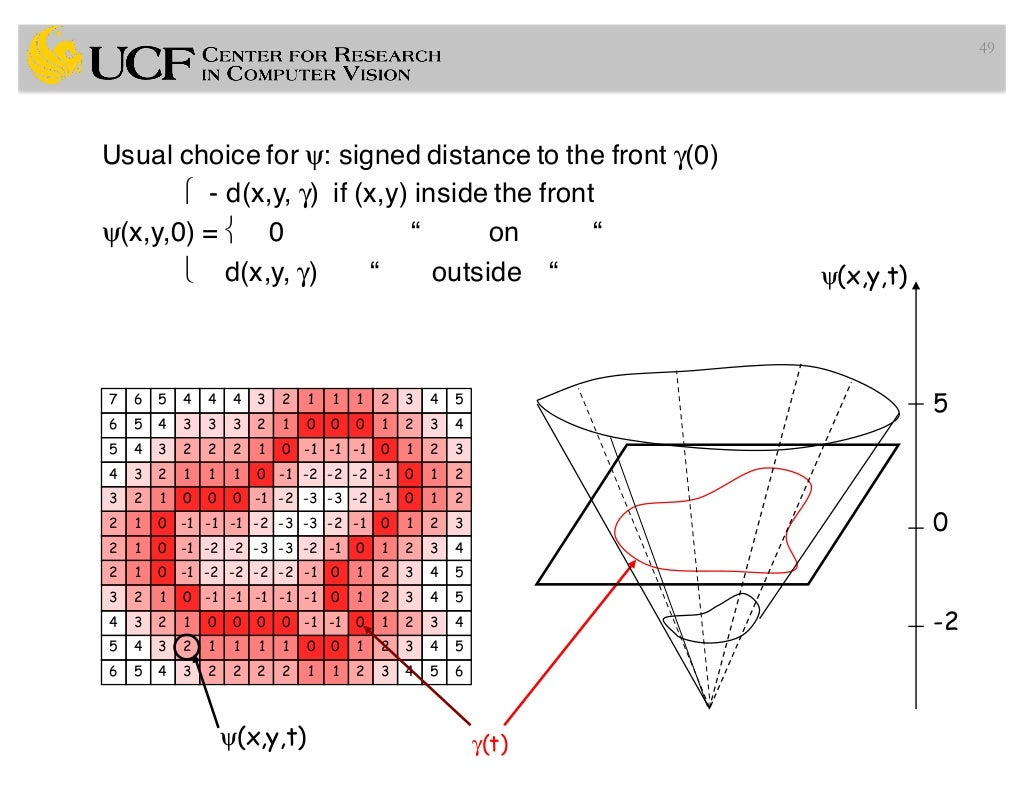
\includegraphics[height=4cm]{Images/level_set_active_contour.jpeg}
        \caption{Courbes de niveaux définissant un contour comme l'intersection de deux courbes implicites.}
        \label{fig:level_set}
      \end{figure}

      Li \cite{Li2011_mri_level_set} utilise les courbes de niveaux pour segmenter des objets malgré une intensité globale non homogène. Pour cela il définit un critère de classification local au voisinage des pixels afin d'estimer un champ de biais d'intensité qui est ensuite incorporé dans l'énergie de propagation.

      \paragraph{Graph cut}

      Une image peut aussi être représentée sous la forme d'un graphe. Dans ce graphe, les nœuds sont les pixels et les arêtes encodent une relation de similarité entre ces derniers. Cette relation peut être spatiale où plus complexe. Dans ce contexte, segmenter un objet ou une région revient à trouver la partition qui maximise la vraisemblance à l'intérieur de chaque ensemble et minimise la vraisemblance entre deux ensembles relativement à un critère (Fig. \ref{fig:graph_cut}).

      \begin{figure}[h]
        \centering
        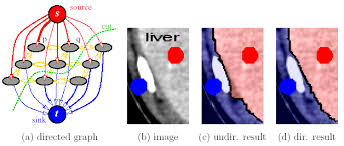
\includegraphics[height=4cm]{Images/graph_cut.jpeg}
        \caption{Principe du graph cut. Une partition est trouvée entre deux régions initialisées chacune par une graine.}
        \label{fig:graph_cut}
      \end{figure}

      Esneault \cite{Esneault2009_moments_graph_cut} utilise les graph cut afin de minimiser une énergie composée de trois critères (région, bordure et vaisseaux). Le modèle de vaisseaux est basé sur un modèle cylindrique.

      Zeng \cite{Zeng2017_liver_oof_graph_cut} propose un raffinement d'une segmentation initiale par graph cut, en utilisant un critère de région basé sur la vraisemblance logarithmique (negative log likelihood) et un critère de bordure basé sur le flux (Sec. \ref{sec:EA:rehaussement:echelle:flux}).

      \paragraph{Ensemble flou}

      Le choix d'une délimitation entre fond et segmentation n'est pas toujours aisé, en particulier dans les images médicales où les bords des objets à segmenter sont assez mal définis. La théorie des ensembles flous permet de modéliser cette incertitude. Au lieu d'associer une classe binaire aux pixels, on associe à chaque pixel une probabilité d'appartenance à chaque classe définie pour le problème donné. Un critère flou est ensuite construit afin de définir une segmentation binaire définitive.

      Sigurosson \cite{Sigurosson2014_retinal_morpho_fuzzy} utilise un ensemble flou pour fusionner l'information provenant de deux ouvertures de chemins pour segmenter les vaisseaux de la rétine. 

      Radojevic et al. \cite{Radojevic2015_fuzzy_logic} détectent les neurones en proposant deux classes floues basées sur le concept de classes multiplicatives. Il définit ensuite le degré d'ambiguïté d'un ensemble flou afin d'attribuer une classe finale aux pixels.
      Zhang et al. \cite{Zhang2018_liver_fuzzy_connectedness} défini un critère de connectivité floue composé d'un critère d'adjacence floue des voxels, et un critère de similarité à la géométrie d'un vaisseau basé sur les filtres de rehaussement de vaisseaux.  

      \paragraph{Deep learning}

      % Better results with deep learning
      Dans les années 2010, un changement de paradigme a lieu avec l'utilisation croissante des réseaux de neurones. En effet, l'apparition des modèles de réseaux profonds, de l'augmentation de la puissance de calculs et d'un nombre important de données annotées ont drastiquement augmenté les performances de ces modèles. Puis, à partir de 2015 les réseaux convolutifs (CNN) prennent une place prépondérante dans la littérature de la segmentation. 
      
      En pratique, on fournit des exemples à un réseau qui produit en réponse une prédiction. L'erreur entre la prédiction et la vérité terrain est ensuite rétro-propagée dans le réseau afin qu'il puisse corriger les prédictions erronées. Ce processus, appliqué de manière itérative sur un grand nombre d'exemples, est appelé entrainement. Deux types d'entraînement sont principalement utilisés, l'entraînement supervisé par paires \{image d'entrée, vérité terrains\} et l'entraînement non supervisé avec des images en entrée et une énergie à minimiser qui permet de contraindre la prédiction du réseau.
      % what is used in medical applications
      Dans le domaine médical, ce sont les réseaux convolutifs complets (FCNN), en particulier l'architecture d'auto-encodeur U-Net \cite{Ronneberger2015_Unet}, qui se sont imposés en permettant de segmenter de manière précise des organes. Ce modèle propose une architecture composée d'un encodeur et d'un décodeur symétriques, donnant au réseau sa forme en U caractéristique. Des \textit{skip connections}, permettent de propager les détails de l'encodeur vers le décodeur.

      Un large panel de variantes de ce réseau a été proposé dans la littérature, combinant ResNet \cite{yu2019_liver_ResUnet}(Fig. \ref{fig:yu_resunet}), DenseNet \cite{Li2018_DenseUnet}, en utilisant plusieurs réseaux travaillant à des résolutions différentes ou en proposant des branches spécialisées.
      
      \begin{figure}[!ht]
        \centering
        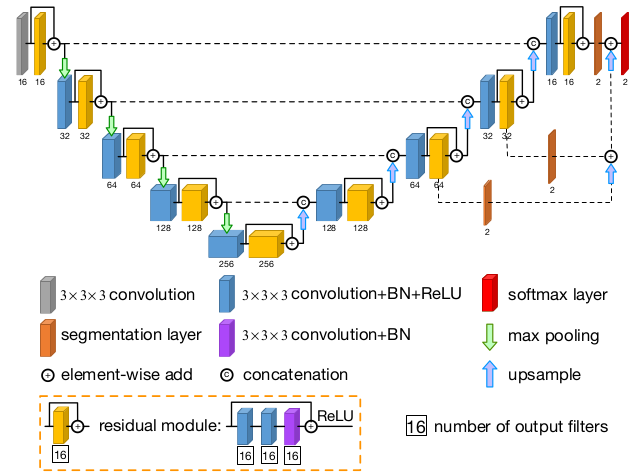
\includegraphics[height=5cm]{Images/Residual_Unet_Yu.png}
        \caption{Architecture \textit{Residual UNet} proposée par Yu et al. \cite{yu2019_liver_ResUnet} pour la segmentation des vaisseaux du foie.}
        \label{fig:yu_resunet}
      \end{figure}
      
      % Loss
      Les résultats des réseaux de neurones sont très dépendants de la fonction de coût qui évalue l'erreur entre la prédiction et les données. Pour la segmentation, la ``Dice loss'' proposée par Sudre \cite{Sudre2017_DiceLoss} s'est popularisée. Cette fonction de coût repose sur le score de Dice qui mesure le recouvrement entre la prédiction et la vérité terrain. Plusieurs métriques similaires ont été proposé et une revue des fonctions de coût pour la segmentation est présentée par Jadon et al. \cite{Jadon2020_survey_seg_loss}. Plus récemment des travaux ont exploré l'introduction de critères topologiques (composantes connexes) afin de limiter la fragmentation des segmentations, particulièrement pertinents pour les structures fines telles que les vaisseaux \cite{Hu2019_topo_homo_persi},\cite{Clough2019_topo_homo_persi},\cite{Ventura2017iterative_topo}. Ces méthodes restent toutefois très coûteuses en temps. 

      Le nombre des données joue un rôle crucial dans la performance des réseaux de neurones. Cependant, nous avons vu dans le chapitre 1 les difficultés de trouver des bases de données publiques avec un nombre important de données bien annotées. 

      Plusieurs méthodes permettent de contourner partiellement ce problème. La plus utilisée est l'augmentation de données \cite{Liskowski2016_data_augmentation}. Celle-ci utilise des données existantes pour appliquer des modifications spatiales ou spectrales des échantillons afin de créer artificiellement des données supplémentaires. D'autres méthodes comptent sur l'utilisation de données partielles, ou d'annotations complètes sur seulement une partie des données \cite{Tajbakhsh2020_imperfect_datasets}. Certains auteurs ont exploré le transfert de style afin de générer des images d'une modalité grâce à des images d'autres modalités. Chartsias et al. \cite{Chartsias2017_heart_adversarial_im} proposent la génération adversaire d'images IRM grâce à des images CT et un masque d'alignement des structures. Chartsias montre qu'en entraînant un réseau sur des images réelles et synthétiques, on augmente les performances d'un réseau de segmentation. Huo et al. \cite{Huo2018_adversarial} explorent la génération à la fois d'une nouvelle modalité et de sa segmentation.

      Ces méthodes peuvent être intéressantes pour le foie dans la mesure où elles peuvent permettre à un réseau d'apprendre la segmentation des vaisseaux en IRM sans les vérités terrains associées (Fig. \ref{fig:ESSNet}).

      \begin{figure}[!ht]
        \centering
        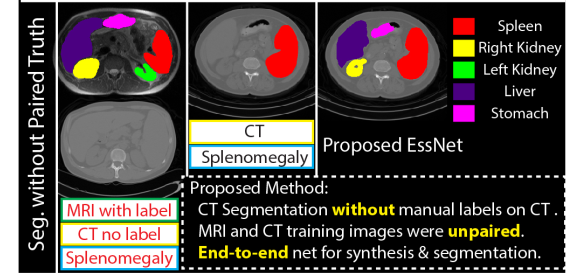
\includegraphics[height=5cm]{Images/ESSNET_application.png}
        \caption{L'apprentissage couplé de la synthèse d'une modalité et de la segmentation associée permet à EssNet (\textit{end-to-end synthesis and segmentation network}) de segmenter une modalité sans annotations manuelles. Travaux de Huo et al. \cite{Huo2018_adversarial}. }
        \label{fig:ESSNet}
      \end{figure}

    \subsubsection{Problématiques de la segmentation}

    Créer une chaîne de segmentation est une tâche complexe. Elle doit apporter des réponses efficaces à la fois à la gestion des artefacts d'acquisition des images, de l'apparence des organes à détecter et de l'extraction d'éléments sémantiques de haut niveau. 

    Les solutions ont été apportées par l'élaboration de chaînes de traitements complexes pour les méthodes sans deep learning. Ainsi, pour la segmentation des vaisseaux hépatiques, Marcan \cite{Marcan2014_vessel_seg} propose un pipeline de segmentation en 16 étapes mélangeant filtrage du bruit, sélection des éléments pertinents par masques et analyses des composantes connexes pour la segmentation des vaisseaux du foie. Goceri \cite{Goceri2017_vessel} propose une méthode en 14 étapes alliant une partion en régions d'intérêt et un étirement du contraste (\textit{contrast stretching}) afin de différencier vaisseaux hépatiques des tissus du foie.
  
    Pour le deep learning, cette complexité se retrouve au niveau de la construction de l'architecture du réseau et de la construction de la base de donnée. Si l'on veut traiter l'information en 3D afin de tirer parti de l'ensemble de la géométrie des vaisseaux, les ressources physiques nécessaires deviennent rapidement un goulot d'étranglement.  
    
    Malgré une littérature dense pour la segmentation vasculaire, illustrée dans les revues de Lesage et al. \cite{Lesage2009_review}, Tankyevych et al. \cite{Tankyevych2011_angiographic} et Moccia et al. \cite{Moccia2018_survey} il n'est pas facile de juger de l'efficacité d'une méthode de segmentation par rapport à une autre. Cette difficulté s'illustre dans les tableaux comparatifs de l'état de l'art conduit par  Moccia (Fig. \ref{fig:moccia_table}) qui montre plusieurs problèmes.

    \begin{figure}[h]
      \centering
      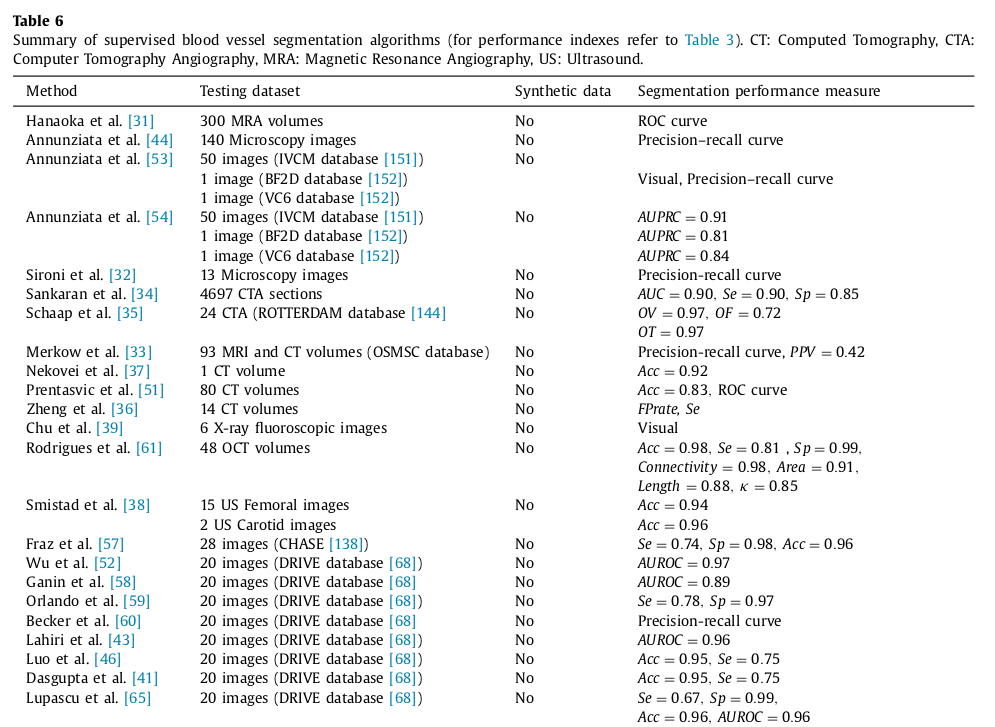
\includegraphics[height=10cm]{Images/Moccia_example.png}
      \caption{Table partielle tirée de Moccia et al. \cite{Moccia2018_survey} récapitulant les résultats de différentes méthodes de segmentation des vaisseaux. Elle illustre la diversité des jeux de données et des méthodes d'évaluations.}
      \label{fig:moccia_table}
    \end{figure}

    Premièrement, il existe une disparité dans les métriques de comparaisons. Certains articles utilisent les métriques standard de classification : précision (\textit{precision}), précision (\textit{accuracy}), sensibilité, spécificité. D'autres travaux utilisent des métriques de recouvrement comme le Dice ou les coefficients de corrélations de Matthew (MCC) et d'autres des opérateurs intégraux de type \textit{Area under curve}(AUC) ou \textit{Receiving Operator}(ROC). Les résultats de certaines méthodes sont mêmes parfois simplement évalués visuellement par des experts.

    Deuxièmement, il y a une hétérogénéité dans les jeux de données. Entre deux articles, il peut y avoir de grandes différences sur le nombre d'images utilisées, les modalités d'acquisition et leur disponibilité. Cette disparité est plus marquée pour les volumes 3D. Des contre-exemples existent comme pour l'imagerie du fond de l'œil (fundus) qui disposent de trois jeux de données annotés qui font référence (DRIVE, STARE, CHASE). L'accessibilité de ces jeux de données annotés est en partie responsable du grand nombre d'articles les utilisant.

    Troisièmement, il est difficile de juger les bénéfices de chaque bloc algorithmique dans une chaîne de segmentation. Une étude ablative où chaque bloc est remplacé afin d'étudier sa performance, comme on pourrait le faire sur les réseaux de neurones, n'est pas forcément possible. Il est donc complexe de juger si les gains obtenus par une méthode sont atteints grâce à sa modélisation du problème, l'utilisation de caractéristiques particulièrement pertinentes, de la métrique permettant une segmentation efficace ou simplement de la paramétrisation judicieuse de l'algorithme.

    En étudiant plus en détail les blocs algorithmiques utilisés pour la segmentation vasculaire traditionnelle, une famille de filtres est utilisée régulièrement en amont des chaînes de traitement. Leur positionnement en fait un élément clé qui conditionne la suite de la segmentation. Ces filtres ont aussi la possibilité d'être appliqués sur les données d'entrées pour le deep learning. Une étude de leurs propriétés nous paraissait donc pertinente comme un premier pas vers la construction d'un algorithme de segmentation.


  \section{Modélisation}

  Les filtres de rehaussement cherchent à isoler et améliorer le signal des structures géométriques associées à des vaisseaux (Fig. \ref{fig:exemple_vesselness}). Ces filtres répondent pour tout ou partie aux objectifs suivants :

  \begin{itemize}
  \item Détecter les structures vasculaires.
  \item Différencier les structures vasculaires des autres structures.
  \item Filtrer les autres structures afin de ne garder que les vaisseaux.
  \item Améliorer le signal des vaisseaux
  \end{itemize}

Les filtres de rehaussement de vaisseaux reposent sur quatre concepts : la modélisation des vaisseaux, le type de caractéristiques utilisées, l'espace d'échelle et la mesure de similarité par rapport au modèle. La modélisation la plus populaire est d'assimiler les vaisseaux à des structures tubulaires. En effet, les vaisseaux sont de longues structures pleines et tortueuses dont la géométrie varie de la ligne (1 voxel de diamètre) à des sections de périmètres irréguliers. Les réseaux vasculaires sont formés par la connections de structures tubulaires qui forment alors une bifurcation. On parle de  bifurcations lorsqu'un vaisseau principal se divise en deux branches, trifurcations en trois et N-furcations dans le cas général. Dans la suite de ce manuscrit, nous effectuons un abus de langage en nommant "bifurcations" l'ensemble des furcations, puisque c'est le cas le plus couramment rencontré. Des hypothèses sont aussi faites sur l'intensité des vaisseaux. Selon les modalités, les vaisseaux peuvent apparaître noirs sur fond plus clair (IRM en phase T1, angiogramme) ou blanc sur fond plus foncé (IRM en phase T2, injection d'agent de contraste). Les hypothèses sont interchangeables, car on peut tout à fait inverser les niveaux de gris de l'image pour passer d'une hypothèse à l'autre. Pour la suite, nous prenons l'hypothèse que les vaisseaux sont clairs sur fond plus sombre.

\begin{figure}[h]
  \centering
  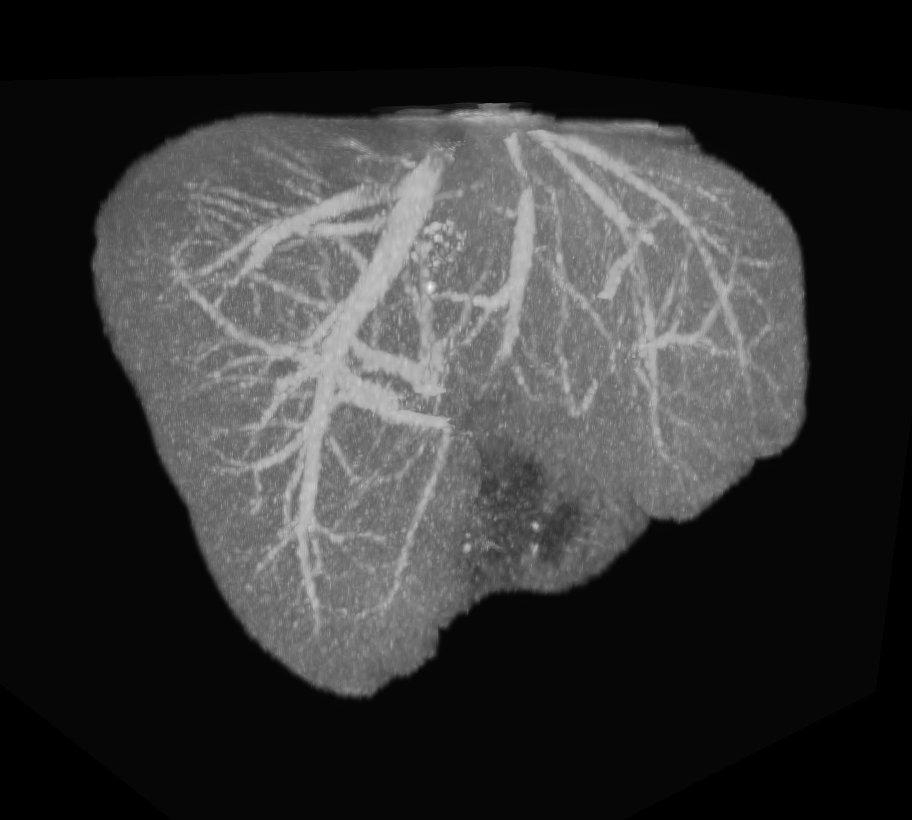
\includegraphics[height=5cm]{Images/enhancement_part1.png}
  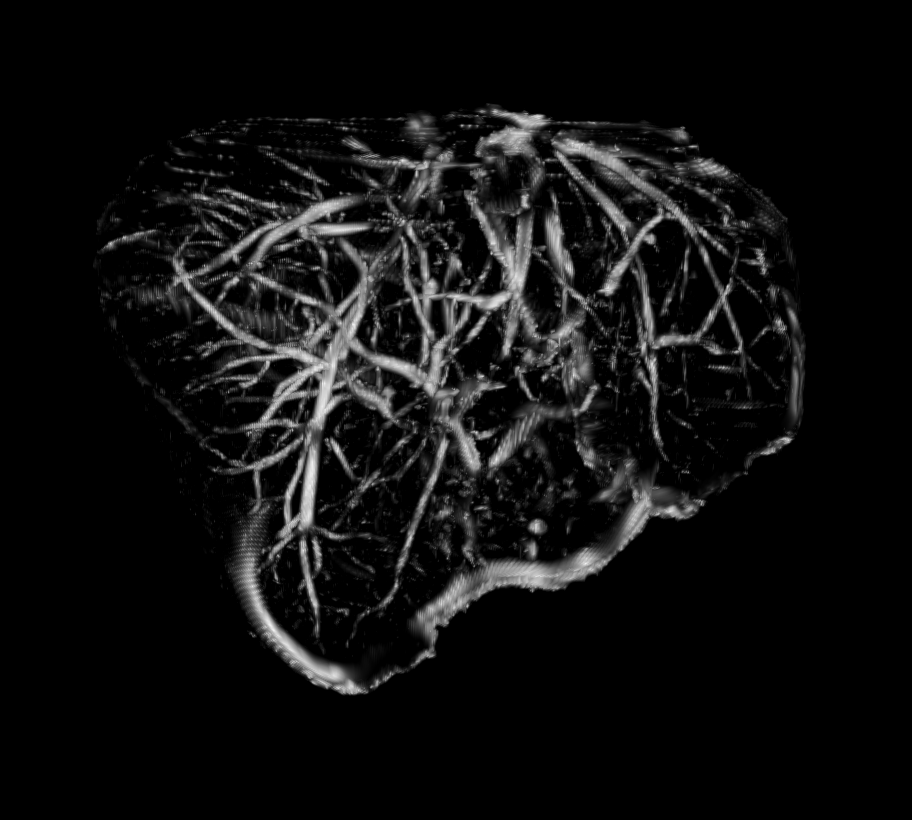
\includegraphics[height=5cm]{Images/enhancement_part2.png}
  \caption{Exemple de filtre de rehaussement de vaisseaux. À droite, un foie en MIP, à gauche les vaisseaux rehaussés. La plupart des vaisseaux inclus dans l'intervalle d'échelle sélectionné sont conservés. Des artefacts de bruit et de bordure sont observables.}
  \label{fig:exemple_vesselness}
\end{figure}

  Avant de définir les caractéristiques utiles à la détection de structures tubulaires, il est nécessaire de définir un espace dans lequel on peut représenter des vaisseaux de tailles différentes dans un cadre commun.

  \section{Espace d'échelles}
  \label{sec:EA:rehaussement:echelle}
  
  La détection d'un réseau vasculaire dans sa totalité implique de détecter des vaisseaux de différentes tailles. En effet, les plus gros vaisseaux peuvent faire plusieurs dizaines de voxels de diamètre tandis que les vaisseaux les plus fins observables, atteignant les limites de la résolution des capteurs, peuvent  mesurer jusqu'à un voxel de diamètre. Il n'est pas envisageable de réécrire un algorithme pour chaque taille de vaisseaux, c'est pourquoi des cadres théoriques, appelés \emph{espace d'échelle} ont été formulés. Ces espaces d'échelles permettent d'établir un cadre uniforme pour sélectionner les structures d'une image à une échelle donnée. Trois espaces d'échelles sont couramment associés au rehaussement vasculaire dans la littérature : l'espace d'échelle gaussien, l'espace d'échelle granulométrique et l'espace d'échelle de flux orienté.
  
  \subsection{Espace gaussien}
  \label{sec:EA:rehaussement:echelle:gaussien}
  Lindeberg introduit la théorie de l'espace d'échelles gaussien dans \cite{Lindeberg1994_scale}. Dans cette théorie, à l'échelle la plus basse, la totalité des structures sont présentes et les détails les plus fins sont présents. Au fur et à mesure que l'échelle augmente, les détails sont lissés pour ne laisser que les maxima locaux correspondant aux formes les plus grandes. Ainsi, l'échelle minimale correspond à l'image initiale et l'échelle maximale correspond à une image uniforme (Fig. \ref{fig:gaussian_smoothing}). Lindeberg a aussi montré que les noyaux gaussiens (Eq. \ref{eq:Gaussienne 3D}) étaient les seuls noyaux permettant de passer d'une échelle fine à une échelle grossière sans provoquer l'apparition de nouvelles structures. Au demeurant, un principe identique a été observé dans le fonctionnement de la vision humaine.
  
  \begin{figure}[!ht]
    \centering
    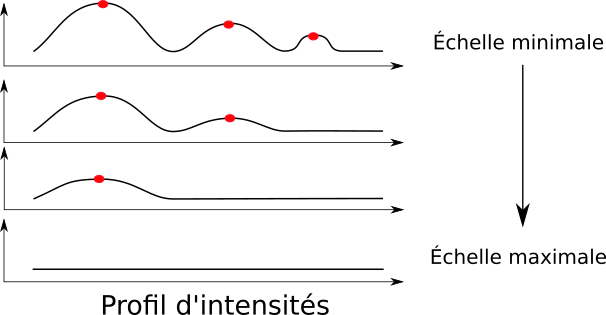
\includegraphics[height=5cm]{Images/gaussian_smoothing.png}
    \caption{Lissage gaussien, les structures de taille égales ou supérieures à $\sigma$ sont conservées alors que les structures de taille inférieures à $\sigma$ disparaissent.}
    \label{fig:gaussian_smoothing}
  \end{figure}
  
  \begin{equation}
    gauss(x,y,z,\sigma_{x},\sigma_{y},\sigma_{z}) = \frac{1}{ \sigma\sqrt{2\pi} }exp(-\frac{x^2 + y^2 + z^2}{2(\sigma_{x}+ \sigma_{y}+ \sigma_{z}) })
    \label{eq:Gaussienne 3D}
  \end{equation}
  
  La sélection de l'échelle dans un espace gaussien se fait par le choix de l'écart-type $\sigma$ de la gaussienne (Fig. \ref{fig:normal_distribution_probability_coverage}). En règle générale, on considère un espace d'échelle avec un lissage uniforme dans toutes les directions : $\sigma_x = \sigma_y = \sigma_z$. Il convient de noter que pour un $\sigma$ donné, le diamètre des structures n'est pas supérieure ou égale à $\sigma$, mais plutôt supérieure ou égale à $\alpha\sigma$. En effet, en empruntant le formalisme des statistiques, l'intervalle de confiance, c'est-à-dire la couverture d'une distribution normale, correspond pour $\sigma=1$ à $34.1$ \percent, $68$ \percent pour $\sigma=2$ et $99.7$ \percent pour $\sigma=3$. Ainsi, pour $\sigma=1$ on détectera en théorie des objets de rayon $3\sigma$ et de diamètre $6\sigma$.  
  
  \begin{figure}[!ht]
    \centering
    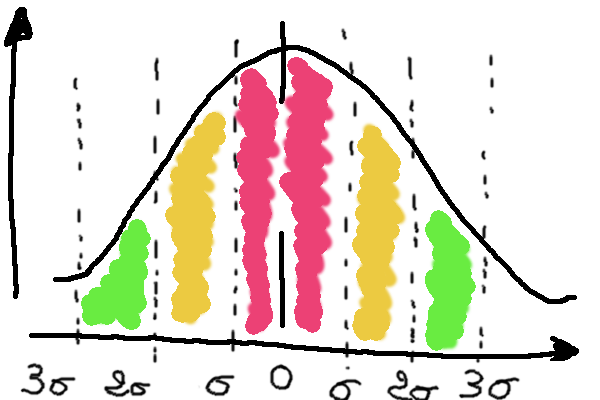
\includegraphics[height=5cm]{Images/normal_distribution_probability_coverage.png}
    \caption{Couverture d'une distribution normale}
    \label{fig:normal_distribution_probability_coverage}
  \end{figure}
  
  L'espace gaussien se prête particulièrement bien à la modélisation des vaisseaux. En effet, la formulation de la gaussienne correspond bien à l'effet combiné des hypothèses de vaisseaux cylindriques et des observations de la diminution d'intensité des vaisseaux au fur et à mesure que l'on s'éloigne de leur centre. En particulier pour un vaisseau parfait de diamètre $3\sigma$, les maxima locaux se situent le long de sa ligne centrale. La justesse de cette hypothèse varie cependant en fonction des modalités et de l'agent de contraste. Le flux sanguin étant parfois laminaire et dans d'autres situations chaotique. La gaussienne se prête aussi très bien à une analyse locale de la géométrie basée sur la dérivation. Elle assure en effet les hypothèses de continuité du support de l'image et permet de combiner lissage et dérivation de l'image en une seule étape par dérivation du noyau gaussien. Enfin, le lissage a l'avantage d'apporter une certaine robustesse au bruit et de compenser la perte locale de signal.

  L'espace gaussien présente cependant des défauts. Le lissage de l'image implique nécessairement un étalement de toutes les structures qui peuvent par conséquent cacher des formes voisines de plus petite taille. Ce phénomène est particulièrement observé lorsque plusieurs échelles sont étudiées. De même, deux structures adjacentes de même taille peuvent fusionner, et ainsi créer une seule réponse, là où deux objets existaient initialement (Fig. \ref{fig:scale_space_spilling}).
  
  \begin{figure}[!ht]
    \centering
    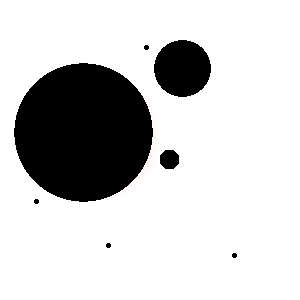
\includegraphics[height=3cm]{Images/gaussian_spilling_init.png}
    
\includegraphics[height=3cm]{Images/gaussian_spilling_g10.png}
    
\includegraphics[height=3cm]{Images/gaussian_spilling_g40.png}
    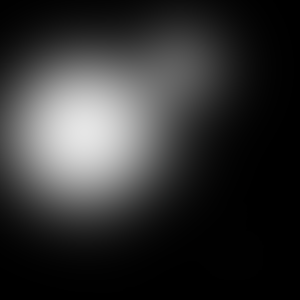
\includegraphics[height=3cm]{Images/gaussian_spilling_g100.png}
    \caption{Débordement du signal des structures larges sur les structures de plus petite taille}
    \label{fig:scale_space_spilling}
  \end{figure}
  
  \begin{figure}[h]
    \centering
    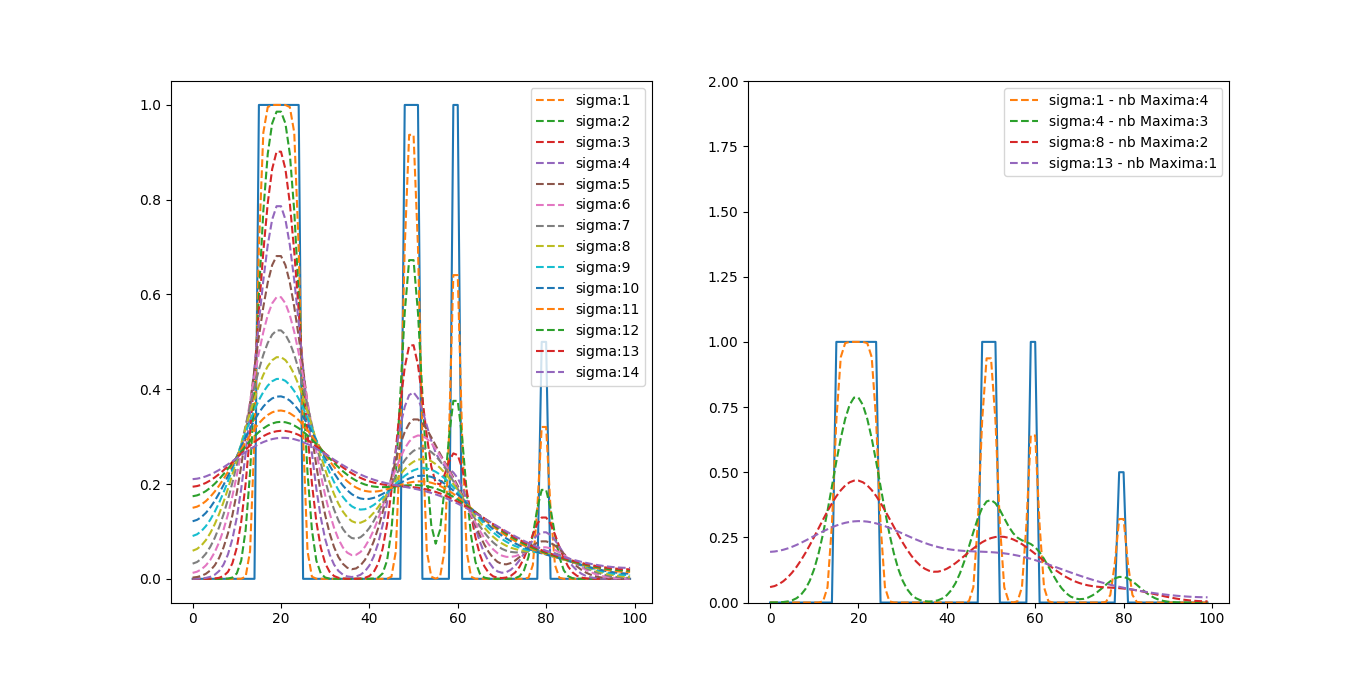
\includegraphics[height=5cm]{Images/GSP_experiment.png}
    \caption{Effet du lissage sur les structures en fonction de $\sigma$. Deux phénomènes sont observés, la fusion et le déplacement des pics des structures adjacentes. Le lissage fait disparaître les structures de faible intensité ou trop fines.}
    \label{fig:scale_space_spilling2}
  \end{figure}
  
  \subsection{Granulométrie}
  \label{sec:EA:rehaussement:echelle:granulometrie}
  
  La granulométrie est l'étude des tailles des particules d'un échantillon. En chimie, on utilise par exemple la technique du tamisage. Elle permet, grâce à un tamis et une grille dont on contrôle la taille du maillage, de ne conserver que des particules dont la taille est trop grosse pour passer à travers le tamis. Un principe similaire est applicable en morphologie mathématique sur les images binaires et par extension en niveau de gris.
  
  \subsubsection{Érosion et dilatation}
  
  Deux opérations élémentaires, la dilatation et l'érosion, permettent de définir les opérations nécessaires pour construire un espace d'échelle morphologique. Les définitions qui vont suivre sont des opérations binaires relatives à des objets blancs sur fond noir.
  
  \paragraph{Définitions}
  % definition de Digital image processing, Gonzalez second edition, Mophology - p518
  
  Soit deux ensembles $A$ et $B$ définis dans $Z^3$ tel que $a=(a_1,a_2,a_3)  \in A$ et $b=(b_1,b_2,b_3) \in B$.
  
  La \emph{translation} de $A$ par $x = (x_1,x_2,x3)$, noté $(A)_x$ est définie par :
  % étrange cette formulation c|c non défini, idem pour x|x dans les autres.
  \begin{equation}
    (A)_x = \{c \mid c = a+x, \forall \text{a} \in A\}. 
    \label{eq:morpho_translation}
  \end{equation}
  On définit la \emph{symétrie} de B, dénoté $\widehat{B}$ par :
  \begin{equation}
    (\widehat{B}) = \{x \mid x = -b, \forall \text{a} \in B\}. 
    \label{eq:morpho_symmetry}
  \end{equation}
  Le \emph{complémentaire} de l'ensemble $A$ est défini par :
  \begin{equation}
    (A^c) = \{x \mid x \not\in A\}. 
    \label{eq:morpho_complementary}
  \end{equation}
  La \emph{différence} de deux ensemble $A$ et $B$, noté $A - B$, est définie par :
  \begin{equation}
    (A-B) = \{x \mid x \in A, x\not\in B \} = A \cap B^c.
    \label{eq:morpho_difference}  
  \end{equation}
  
  \paragraph{Dilatation}
  En utilisant les propriétés précédentes, la dilatation s'exprime de la manière suivante :
  \begin{equation}
    A \oplus B = {a+b \mid b \in B, a \in A } = \bigcup_{a \in A}B_{a} \
  \end{equation}
  %\begin{equation}
  % A \oplus B = \{x \mid (\widehat{B}_x, \cap A \neq \emptyset) \}
  %\end{equation}
  La dilatation de $A$ par $B$ est l'ensemble de tous les déplacements de $\widehat{B}$ tel qu'il y a au moins un pixel de recouvrement entre $A$ et $\widehat{B}$. Cette opération permet de faire grossir une structure en fonction de la forme de B \ref{fig:morpho_dilation}.
  
  \begin{figure}[h]
    \centering
    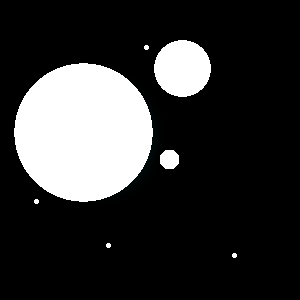
\includegraphics[height=3cm]{Images/morpho_init.png}
    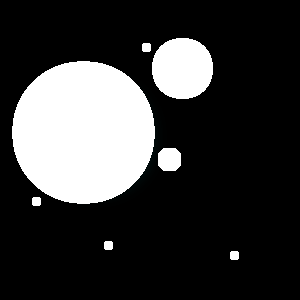
\includegraphics[height=3cm]{Images/morpho_dilate_k5.png}
    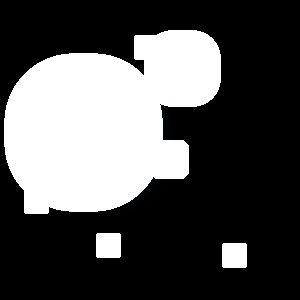
\includegraphics[height=3cm]{Images/morpho_dilate_k21.png}
    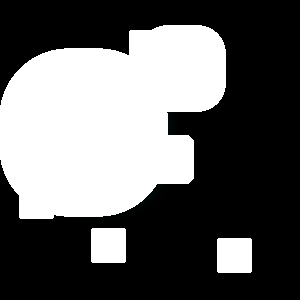
\includegraphics[height=3cm]{Images/morpho_dilate_k31.png}
    \caption{Exemple de dilatation par un élément structurant rectangulaire. La dilatation fait grossir les structures selon la forme de l'élément structurant.}
    \label{fig:morpho_dilation}
  \end{figure}
  
  L'ensemble $B$ est couramment appelé \emph{élément structurant}. 
  \todo{"indiquer qu'en général, il contient 0 afin d'éviter des effets de translation dans l'image résultat" Je ne comprends pas bien ce que cela implique. On parle d'une ancre ou d'avoir des zéros dans l'élément structurant ?}
  
  \paragraph{Érosion}
  L'opération opposée à la dilatation est l'érosion (Fig. \ref{fig:morpho_erosion}).
  \begin{equation}
    A \ominus B = \{x \mid (B)_x, \subseteq A\}
  \end{equation}
  L'érosion de $A$ par $B$ est l'ensemble de tous les points $x$ tel que $B$ translaté de $x$ est inclus dans $A$. 
  
  \begin{figure}[h]
    \centering
    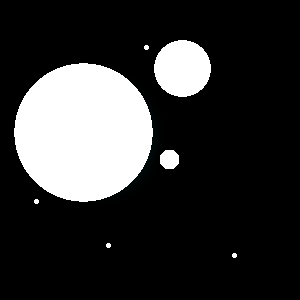
\includegraphics[height=3cm]{Images/morpho_init.png}
    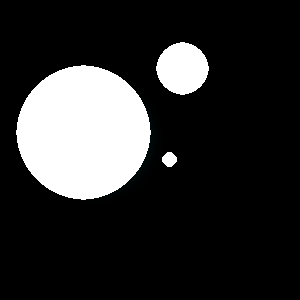
\includegraphics[height=3cm]{Images/morpho_erode_k5.png}
    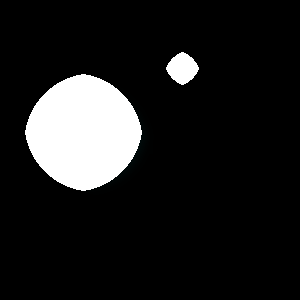
\includegraphics[height=3cm]{Images/morpho_erode_k21.png}
    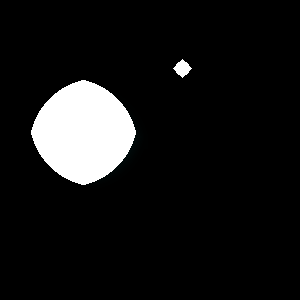
\includegraphics[height=3cm]{Images/morpho_erode_k31.png}
    \caption{Exemple d'érosion avec un élément structurant rectangulaire. L'érosion peut faire disparaître des petites structures et érode les structures en fonction de la géométrie de l'élément structurant.}
    \label{fig:morpho_erosion}
  \end{figure}
  
  \subsubsection{Fermeture et ouverture}
  À partir des opérations d'érosion et de dilatation, on peut définir des opérations composites : l'ouverture et la fermeture.
  \paragraph{Fermeture}
  L'ouverture est définie comme la dilatation de $A$ par $B$ suivi de l'érosion du résultat par $B$.
  \begin{equation}
   A \bullet B = (A \oplus B) \ominus B
  \end{equation}  
  Cet opérateur est utilisé pour boucher les trous dont la surface est inférieure à la surface de l'élément structurant (Fig. \ref{fig:morpho_femerture}). L'érosion qui suit la dilatation permet d'assurer que la taille reste stable.
  
  \begin{figure}[h]
    \centering
    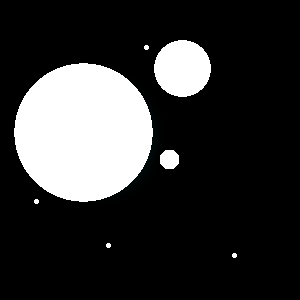
\includegraphics[height=3cm]{Images/morpho_init.png}
    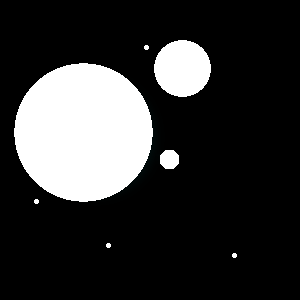
\includegraphics[height=3cm]{Images/morpho_close_k5.png}
    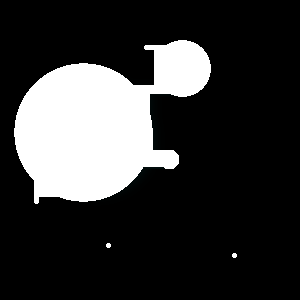
\includegraphics[height=3cm]{Images/morpho_close_k21.png}
    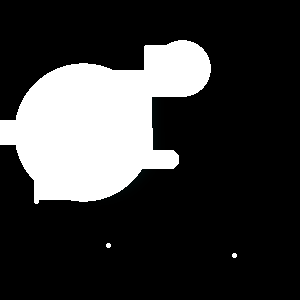
\includegraphics[height=3cm]{Images/morpho_close_k31.png}
    \caption{Exemple de fermeture par un élément structurant rectangulaire. La fermeture reconnecte des éléments adjacents en fonction de la géométrie de l'élément structurant.}
    \label{fig:morpho_femerture}
  \end{figure}
  
  \paragraph{Ouverture}
  L'ouverture est définie comme l'érosion de $A$ par $B$ suivie de la dilatation du résultat par $B$.
  \begin{equation}
   A \circ B = (A \ominus B) \oplus B
  \end{equation}
  \begin{figure}[h]
    \centering
    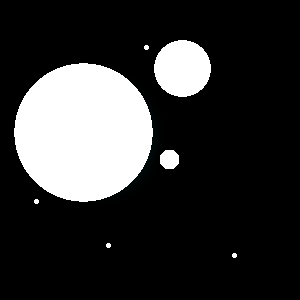
\includegraphics[height=3cm]{Images/morpho_init.png}
    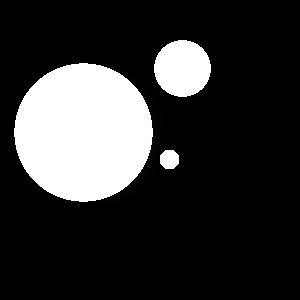
\includegraphics[height=3cm]{Images/morpho_open_k5.png}
    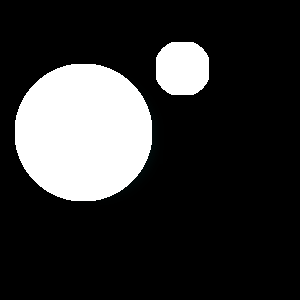
\includegraphics[height=3cm]{Images/morpho_open_k21.png}
    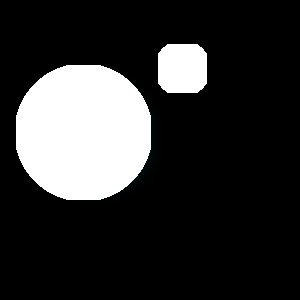
\includegraphics[height=3cm]{Images/morpho_open_k31.png}
    \caption{Exemple d'ouverture}
    \label{fig:morpho_ouverture}
  \end{figure}
  Cet opérateur est utilisé pour supprimer les structures de tailles inférieures à la surface de l'élément structurant (Fig. \ref{fig:morpho_ouverture}). La dilatation qui suit l'érosion permet d'assurer que la taille des éléments restent stable. L'ouverture permet de construire un espace d'échelle paramétré par la taille de l'élément structurant. Cet espace ne souffre pas d'une fusion parasite des structures adjacentes.
  
  \subsection{Flux}
  \label{sec:EA:rehaussement:echelle:flux}
  
  Comme nous l'avons vu dans la section \ref{sec:EA:rehaussement:echelle:gaussien}, l'espace d'échelle gaussien peut provoquer des débordements de structures sur d'autres, plus petites. On peut limiter ce problème en utilisant un cadre différent, celui de l'analyse des flux.
  
  Si l'on considère un champ de vecteur $V$, par exemple un fluide ou un champ de gradient pour une image, on définit le flux (Eq. \ref{eq:flux}) passant à travers la surface $S$, orienté par sa normale $\vec{n_s}$, comme l'intégrale de la somme du produit scalaire entre le vecteur de flux $\vec{v}$ et la normale à la surface $\vec{n}$.
  
  \begin{equation}
  flux_S = \int_{S}< \vec{v},\vec{n} > d\rho
  \label{eq:flux}
  \end{equation}
  
  On peut appliquer le calcul de flux à la surface d'un objet fermé. En particulier, des structures en forme de disques ou de sphères ont été particulièrement utilisées pour l'analyse de vaisseaux sanguins. On peut en effet contrôler directement le diamètre d'une sphère pour détecter les objets de la taille voulue. Cette formulation de l'échelle diffère des méthodes précédentes, car les objets tubulaires ne sont détectés que pour une échelle donnée, là où les deux autres techniques conservent les objets à l'échelle donnée et aux échelles supérieures. Elle a aussi l'avantage de limiter l'analyse du flux à la surface de la sphère et donc de produire une réponse qui ne déborde pas.
  
  La précision du calcul de l'intégrale de flux dépend du nombre d'échantillons effectués sur $S$. Plus celui-ci est grand, plus le calcul est coûteux. De plus, plus l'échelle sélectionnée est grande, et donc plus la surface de la sphère est grande, plus le nombre d'échantillons requis est important. Law propose une formulation élégante du calcul de flux dans le domaine de Fourier afin de réduire drastiquement le temps de calcul par rapport à l'implémentation naïve \cite{Law2009_efficient_implementation}.
  Pour y parvenir, Law propose d'exprimer le calcul de flux sous la forme d'une convolution dans le domaine temporel. L'avantage de la convolution est double : on évite l'étape d'échantillonnage sur la surface et la convolution s'exprime comme une multiplication dans le domaine de Fourier. On peut exprimer le calcul de flux en termes de volume et non plus en termes de surface grâce au théorème de la divergence qui établit une égalité entre le flux à la surface d'un objet et le flux à l'intérieur de son volume. Ainsi :
  \begin{equation}
    flux_{\partial C} = \int_{\partial C}< \vec{v},\vec{n} > d\rho \equiv \int_{C }\Delta I d\nu
  \end{equation}
  Plus précisément :
  \begin{equation}
    f_s(x,y,z) = \int_{R_s}\vec{v}(x+t,y+p, z+q) . \vec{n}_{(t,p,q)}dA
    \label{eq:next_oof}
  \end{equation}
  avec $R_s$ une région sphérique de rayon $s$, $dA$ une surface infinitésimale sur la surface $\partial R_s$, $\vec{n}_{(t,p,q)}dA$ le vecteur normal à $dA$ à la position $(t,p,q)$ et $\vec{v}$ le gradient de l'image $I$. $\vec{v}$ est obtenu à partir de l'image $I$ lissée par un noyau gaussien afin d'assurer la dérivabilité du signal de $I$. $\vec{v}=\nabla(g*I)$.
  Eq. \ref{eq:next_oof} est équivalent à :
  \begin{align}
    f_s(x,y,z) & = \int_{R_s} \vec{div}( \vec{v}(x+t,y+p, z+q) ) dtdpdq \\
    & = \int_{\omega} d_s(t,p,q) [\vec{div}( \vec{v}(x+t,y+p, z+q) )] dtdpdq
  \end{align}
  où $\omega$ est le domaine entier de l'image et $d_s(t,p,q)$ correspond à la fonction porte sphérique définie par :
  \begin{align}
    d_s(x,y,z) & = \begin{cases} 
                  1, \sqrt{x^2 + y^2 + z^2} \leq s  \\
                  0, \text{sinon} \\
                \end{cases}
  \end{align}
  Ainsi, $f_s(x,y,z)$ peut être exprimé sous forme de convolution :
  \begin{align}
    f_s(x,y,z) & = \int_{\omega} d_s(t,p,q) [\vec{div}( \vec{v}(x+t,y+p, z+q) )] dtdpdq \\
               & = \int_{\omega} d_s(t,p,q) (\Delta(g*I(x+t,y+p, z+q)))] dtdpdq \\
               & = \int_{\omega} d_s(-t,-p,-q) (\Delta(g*I(x+t,y+p, z+q)))] dtdpdq \\
               & = d_s * \Delta g * I(x,y,z) \\
               & = I * h_s(x,y,z) \\
    \label{eq:oof_next2}
  \end{align}
  avec $*$ l'opérateur de convolution, $\Delta$ l'opérateur laplacien.
  Eq. \ref{eq:oof_next2} exprimé dans le domaine de Fourier donne :
  \begin{align}
    FFT( I * h_s(x,y,z) ) &= FFT(I) . H_s(u,v,w) \\
                         &= FFT(I) . [ (j2 \pi)^2 ( (\frac{u}{N_x})^2 + (\frac{v}{N_y})^2 + (\frac{w}{N_z})^2 ) ] \\
                         & . [ exp( -( (\frac{u}{N_x})^2 + (\frac{v}{N_y})^2 + (\frac{w}{N_z})^2 ) 2(\pi\sigma)^2 ) ]
  \end{align}
  \begin{figure}[!ht]
    \centering
    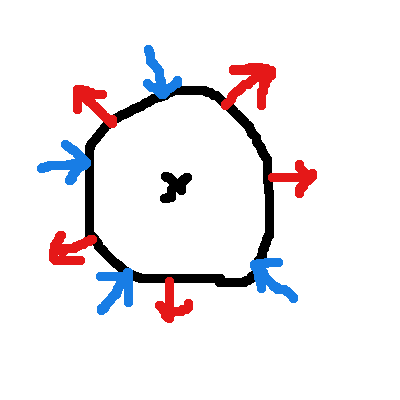
\includegraphics[height=6cm]{Images/flux.png}
    \label{fig:flux_sphere}
    \caption{flux sur la surface d'une sphère. Dans une image, maximiser le flux (gradient) sortant de la sphère revient à positionner celle-ci au centre d'un vaisseau.}
  \end{figure}
  \subsection{Multi-échelle}
  \label{sec:EA:rehaussement:echelle:multiScale}

  Les résultats des filtres de rehaussement appliqués à différentes échelles sont rarement traités séparément. À la place, ils sont fusionnés dans une seule et même réponse grâce à un opérateur max. Cet opérateur permet de récupérer pour un pixel donné la réponse maximale à travers l'ensemble des échelles
  
  \begin{equation}
    V(I)_{multi echelle} = max_{\sigma}V_{\sigma}(I)
  \end{equation}
  
  Cet opérateur peut provoquer un recouvrement des structures adjacentes par une structure ayant une réponse plus haute. À notre connaissance, aucune publication ne propose de pondérer ou de hiérarchiser la réponse en fonction de la taille du noyau (gaussienne, élément structurant, sphère, etc.) de l'espace d'échelle.

  Le choix de l'intervalle d'un espace multi-échelle est contrôlé par une borne inférieure, une borne supérieure et un nombre d'échelles dans cet intervalle. De manière naïve, on pourrait choisir d'espacer les échelles individuelles de manière équidistante sur l'intervalle. Pour les vaisseaux, plus ceux-ci sont fins et plus leur densité augmente. Il est donc nécessaire de consacrer un plus grand nombre d'échelles basses et un nombre plus réduit d'échelles hautes pour capturer efficacement l'ensemble des réseaux vasculaires. On préfère donc utiliser un espace d'échelles logarithmique à un espace d'échelles linéaire (Fig. \ref{fig:scale_space}).

  \begin{figure}[h]
    \centering
    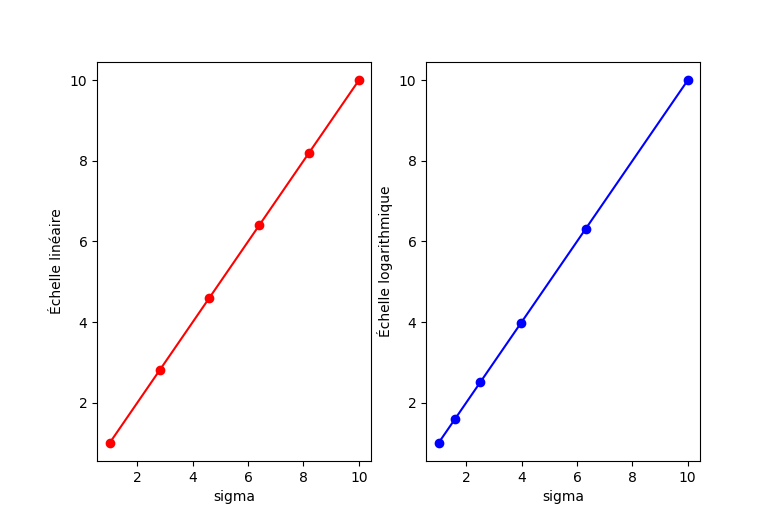
\includegraphics[height=6cm]{Images/scale_space.png}
    \caption{Espace d'échelles linéaire vs espace d'échelles logarithmique : $borne_{inf}=1,borne_{sup}=10,échelles=10$. Avec l'échelle logarithmique, les variations des petits vaisseaux sont mieux capturés.}
    \label{fig:scale_space}
  \end{figure}

\section{Caractéristiques}

La différenciation entre les vaisseaux et d'autres structures s'effectue à l'aide de caractéristiques extraites de l'image qui permettent de définir localement la géométrie autour d'un pixel. 

\subsection{Morphologie}
\label{sec:EA:rehaussement:morpho}

Le rehaussement à base d'opérateurs morphologiques s'articule autour de deux familles, la composition d'éléments structurants rigides et l'utilisation de chemins curvilinéaires flexibles.

La composition d'éléments structurants rigides s'effectue la plupart du temps avec des boules et des cylindres. Les cylindres permettent de couvrir les parties curvilignes des vaisseaux, tandis que les boules couvrent les jonctions. Une composition d'ouvertures avec ces éléments est ensuite utilisée pour récupérer le réseau vasculaire. Sazak propose un schéma de ce type en 2D \cite{Sazak2019_bowler_hat_2D} et en 3D \cite{Sazak2018_bowler_hat_3D} et compare son efficacité relativement au rehaussement à base de tenseurs de phase et hessien. Cette méthode bien que simple à mettre en pratique, nécessite plusieurs itérations avec des rotations des éléments structurants afin de capturer toutes les orientations des structures tubulaires. Elle peut ainsi rapidement devenir coûteuse en 3D.

\begin{figure}[h]
  \centering
  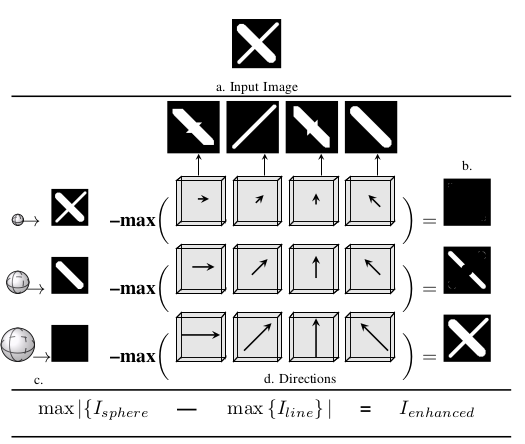
\includegraphics[height=4cm]{Images/bowlerHat_3D.png}
  \caption{\textit{Bowler hat transform} proposée par Sazak et al. La combinaison d'éléments sphériques et linéaires permet de capturer les structures curvilinéaires. }
  \label{fig:sazak_bowler_hat}
\end{figure}

L'un des défauts de la méthode précédente est le caractère fixe des éléments structurants qui ne permettent pas toujours de capturer les variations de formes des vaisseaux. Hejimans \cite{Heijmans2005_path_opening} propose une famille d'éléments structurants variable dont la forme est définie par une grille d'adjacences. Des améliorations successives de cet algorithme ont été proposé : Cokelaer et al. \cite{Cokelaer2012_efficient_path_opening} proposent une version robuste au bruit en autorisant des discontinuités dans l'élément structurant, Van de Gronde \cite{Gronde2015_fast_path_opening} propose une implémentation efficace de l'algorithme en $o( N log ( L ))$ avec $N$ le nombre de pixels de l'image et $L$ la taille du chemin. Enfin Merveille et al. \cite{Merveille2018_curvilinear} itèrent sur la méthode en proposant un classement de l'orientation des chemins afin de segmenter les vaisseaux dans des images 2D et 3D (voir Sec. RORPO). 


\subsection{Phase}
\label{sec:EA:rehaussement:Phase}

Une image peut-être à la fois vue comme une matrice de pixels et comme un signal discret en 2 ou 3 dimensions. Lorsque l'on considère la représentation sous forme de signal on peut décomposer celui-ci en deux éléments indépendants : l'amplitude, correspondant à l'intensité des pixels et la phase, correspondant à la distance entre deux pics de deux signaux. La phase étant une mesure relative à la position des pics, elle ne prend pas en compte l'amplitude de ceux-ci et présente donc une invariance aux changements d'intensités. Oppenhei et al. \cite{Oppenheim1981_phase_importance} démontrent l'importance de ces caractéristiques de l'image et montre une correspondance avec le système visuel humain. 

\begin{figure}[h]
  \centering
  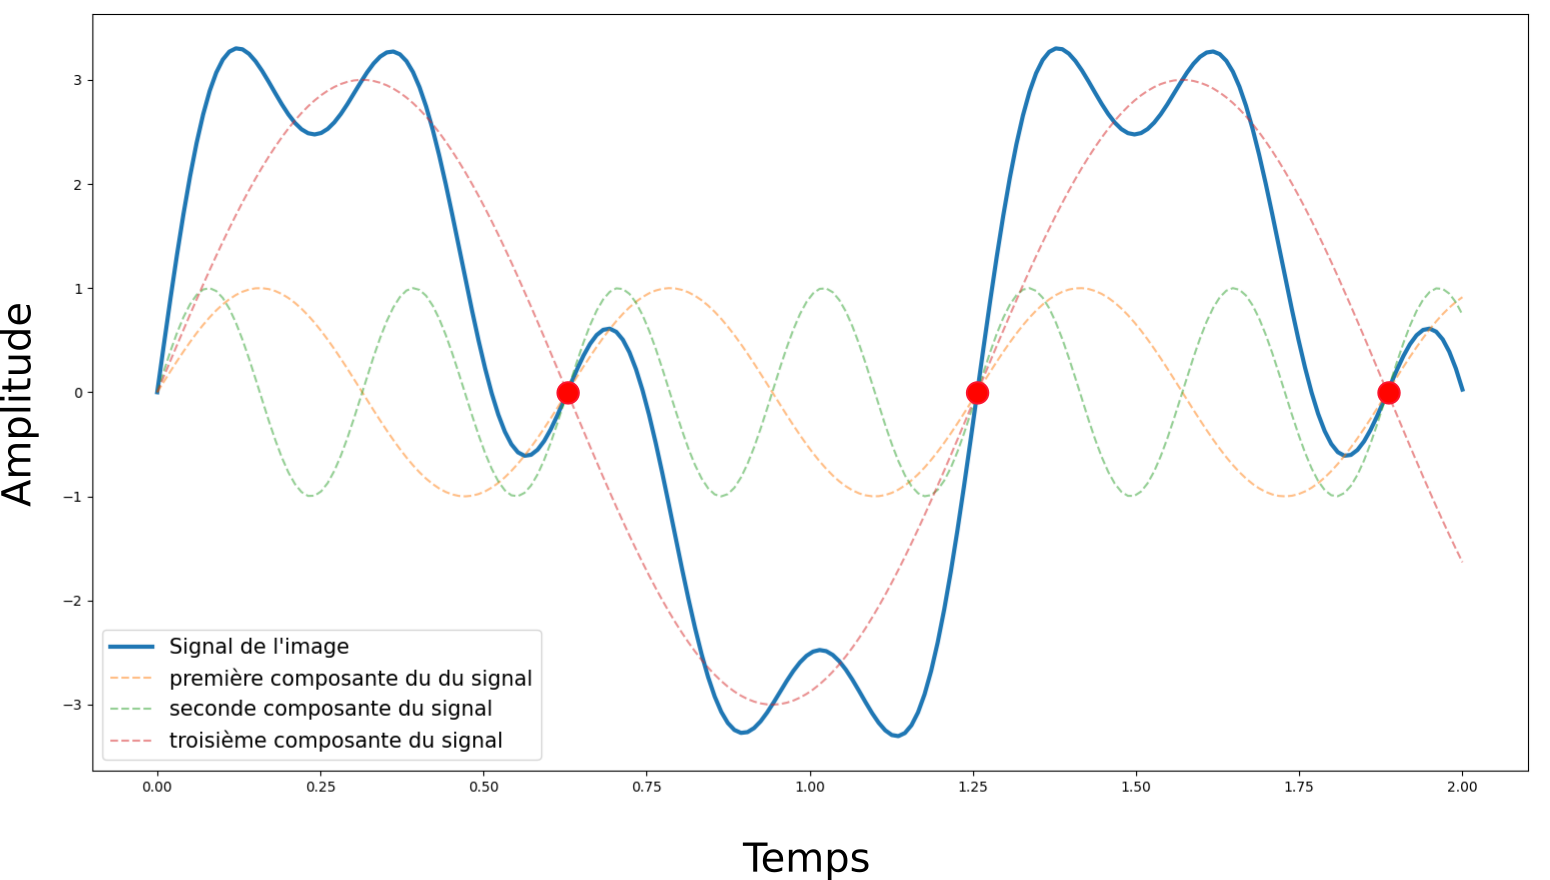
\includegraphics[height=5cm]{Images/PC_decomposition.png}
  \caption{Décomposition de Fourier d'un signal, en certains points la phase de chaque composant est synchronisée}
  \label{fig:phase congruency}
\end{figure}

Plusieurs constructions de filtres de rehaussement se basent sur cette propriété pour la détection des vaisseaux. Obara et al. \cite{Obara2012_phase} utilisent un tenseur de structure basé sur le contraste de phase. Les valeurs propres de ce tenseur permettent ensuite d'exprimer une mesure de tubularité.

Ce tenseur est exprimé comme :

\begin{equation}
  T_{PC} = \sum PC_{o}(p)(n_{o}n^T - \alpha \text{I})
\end{equation}

Avec $PC(x)$ la fonction de congruence de phase, $n_{\theta}=[cos(\theta),sin(\theta)]^T$ le vecteur d'orientation $o$, $I$ le tenseur unitaire, $\alpha = 1/(m-1)$ avec $m$ la dimension de $I$. $PC(x)$ permet de détecter les éléments saillants à la manière d'un détecteur de contours.
En effet, une image vue comme un signal peut être décomposée comme un ensemble de signaux sinusoïdaux. Les éléments saillants tels que les bordures ou les coins d'objets correspondent à une synchronisation, e.g congruence, de ces signaux pour un angle donné. La congruence de phase s'exprime par :

\begin{equation}
  PC(x) = max_{\theta \in [0,2\pi)} \sum  \frac{ \alpha_{\omega}cos(\omega x + \phi_{\omega} - \omega)  }{ \alpha_{\omega}d \omega } d \omega
\end{equation}

Elle représente la variance de phase des différents signaux au point $x$. Lorsque les phases des signaux sont égales, $PC(x)=1$.
En pratique, cette définition est complexe à implémenter. On lui préfère en la mesure d'énergie locale qui s'approxime avec des filtres de Gabor ou des ondelettes. Ces filtres sont basés sur des gaussiennes dont on peut contrôler l'échelle comme un espace gaussien.

\begin{figure}[h]
  \centering
  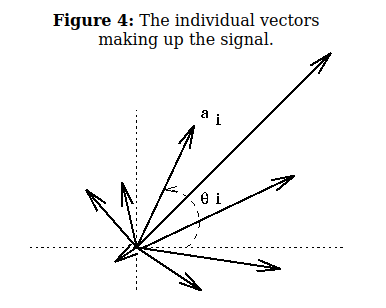
\includegraphics[height=5cm]{Images/PC_vectors.png}
  \caption{Représentation vectorielle d'un signal, chaque vecteur représente une composante sinusoïdale paramétrée par sa phase pour l'orientation et son amplitude pour sa norme. Des signaux congruents sont des signaux dont les angles des vecteurs sont similaires.}
  \label{fig:phase_congruency_vectors}
\end{figure}

Enfin, ces filtres sont dépendants du nombre d'orientations échantillonnées $\omega$. En pratique entre 6 et 10 échantillons régulièrement espacés suffisent. 

\subsection{Hessienne}
\label{sec:EA:rehaussement:hessienne}

La matrice hessienne est la matrice des dérivées secondes de l'image en un pixel (Eq. \ref{eq:hessian_matrix}). Celle-ci permet d'exprimer la courbure locale autour d'un point.
Les valeurs propres et vecteurs propres de la hessienne permettent de quantifier l'orientation, le sens et l'amplitude du voisinage d'un point (Fig. \ref{fig:structures_hessienne}).
La simplicité de la hessienne a permis l'émergence de nombreuses modélisations de rehaussement.
\begin{equation}
  H(f) =
  \begin{bmatrix}
  h_{11} & h_{12} & h_{13} \\
  h_{21} & h_{22} & h_{23} \\
  h_{31} & h_{32} & h_{33} \\
  \end{bmatrix}
    =
  \begin{bmatrix}
  \frac{\partial^2 f}{\partial x^2_1} & \frac{\partial^2 f}{\partial x_1 \partial x_2} & \frac{\partial^2 f}{\partial x_1 \partial x_3} \\
  \frac{\partial^2 f}{\partial x_2 \partial x_1} & \frac{\partial^2 f}{\partial x^2_2} & \frac{\partial^2 f}{\partial x_2 \partial x_3} \\
  \frac{\partial^2 f}{\partial x_3 \partial x_1} & \frac{\partial^2 f}{\partial x_3 \partial x_2} & \frac{\partial^2 f}{\partial x^2_3} \\
  \end{bmatrix}
  \nonumber
  \label{eq:hessian_matrix}
\end{equation}
\begin{figure}[!ht]
  \centering
  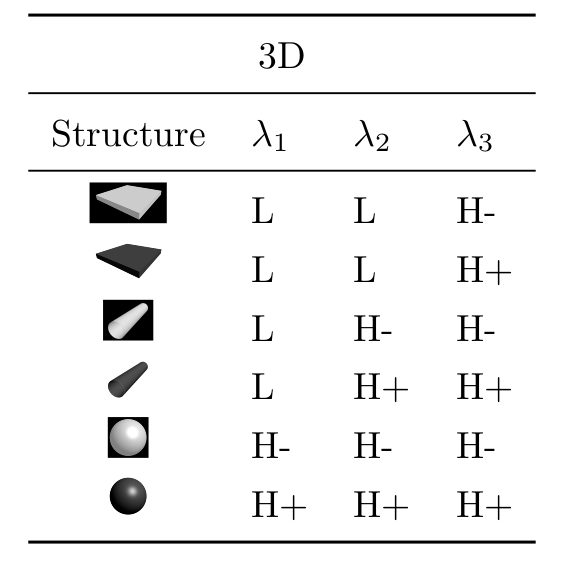
\includegraphics[height=4cm]{Images/table_structures_jerman.png}
  \caption{Description de la géométrie locale par les valeurs propres de la hessienne. source:\cite{Jerman2015_beyond_frangi}.}
  \label{fig:structures_hessienne}
\end{figure}

\section{Mesures de tubularité}
\todo{Est-ce qu'on s'attend à une discussion sur les termes de chaques vesselness ou a minima à des illustrations de chaque vesselness ?}
En 3D, une structure tubulaire parfaite peut-être exprimée par les valeurs propres. Soit $\lambda_1$,$\lambda_2$,$\lambda_3$ tels que $|\lambda_1| \leq |\lambda_2| \leq |\lambda_3|$.  En termes de valeurs propres, la tubularité peut s'exprimer de la manière suivante \cite{Lorenz1997_multi} :
\begin{align}
  \lambda_1 \approx 0 \\
  \lambda_1 \ll \lambda_2 \\
  \lambda_2 \approx \lambda_3
\end{align}
Ces équations sont valables dans un contexte spécifique. Lorsque le $\sigma$ de l'espace d'échelle coïncide avec la taille d'une structure tubulaire, la ligne centrale de celle-ci devient un maximum local. Le vecteur propre $\lambda_1 \approx 0$ correspond à la direction du tube. Dans ce cas, l'amplitude $\lambda_1$ est proche de zéro car le gradient dans cette direction est presque nul. Dans les deux directions principales de la coupe, l'intensité du tube décroissant rapidement au fur et à mesure que l'on s'éloigne du centre, les valeurs propres $\lambda_2$ et $\lambda_3$ sont donc élevées.

\subsection{Sato}

Sato \etal \cite{Sato1998_vesselness} sont parmi les premiers à se servir de cette formulation. (N.B. : l'ordonnancement des valeurs propres est légèrement différent pour Sato. On définit $\lambda^\star_i$ tel que $\lambda^\star_1 \geqslant \lambda^\star_2  \geqslant  \lambda^\star_3$.)
Quand $\lambda^\star_2, \lambda^\star_3 < 0$, le vecteur propre $\mathbf {e^\star_1}$ associé à $\lambda^\star_1$ pointe dans la direction de la plus petite variation d'intensité, qui est aussi la direction du vaisseau.
Dans ce cas les vecteurs propres $\mathbf {e^\star_2}$ et $\mathbf {e^\star_3}$ forment une base orthogonale à $\mathbf {e^\star_1}$ et correspondent à la tranche du vaisseau.
La taille des axes de la tranche des vaisseaux est proportionnelle à $|\lambda^\star_2|$ et $|\lambda^\star_3|$.

Le filtre de rehaussement de Sato utilise un ratio asymétrique de valeurs propres pour obtenir une réponse forte sur les structures tubulaires, basé sur le signe de $\lambda^\star_1$.
Ce filtre à l'avantage de lisser la réponse et de réduire le bruit. Deux paramètres $\alpha_1$ et $\alpha_2$ contrôlent la force de cette asymétrie :
\begin{equation}
\nonumber
F =
\left\{
\begin{array}{lr}
\lambda^\star_c \exp(-\frac{{\lambda^\star_1}^2}{2(\alpha_1 \lambda^\star_c)^2})  & \lambda^\star_1 \leqslant 0, \lambda^\star_c \neq 0 \\
\lambda^\star_c \exp(-\frac{{\lambda^\star_1}^2}{2(\alpha_2\lambda^\star_c)^2})  &  \lambda^\star_1 > 0, \lambda^\star_c \neq 0 \\
0 & \quad \lambda^\star_c = 0
\end{array}
\right.
\end{equation}
Avec $\lambda^\star_c = \min\{-\lambda^\star_2,-\lambda^\star_3\}$.

\subsection{Frangi}

Une année plus tard, Frangi \etal \cite{Frangi1998_vesselness} exploitent l'ensemble des valeurs propres afin de proposer un contrôle plus fin sur la géométrie des motifs rehaussés. Trois mesures sont dérivées des valeurs propres :
\begin{align}
 \nonumber
  R_b & = |\lambda_1| / \sqrt{|\lambda_2\lambda_3|}\\
R_a & = |\lambda_2| / |\lambda_3| \nonumber\\
S & = \sqrt{\lambda^2_1 + \lambda^2_2 + \lambda^2_3} \nonumber
\end{align}
Ces mesures permettent de discriminer les blobs ($R_b$), différencier les plateaux des structures en ligne ($R_a$) et contrôler les structures de faible contraste en étudiant la norme de la hessienne ($S$). C'est trois mesures sont unifiées dans une fonction de rehaussement :   

\begin{align}
  F & = \begin{cases} 
                \big(1-\exp\big(-\frac{R_a^2}{2\alpha^2}\big)\big) \exp\big(-\frac{R_b^2}{2\beta^2}\big)\big(1-\exp(-\frac{S^2}{2C^2}\big)\big), \text{Si} \lambda_2, \lambda_3 \leqslant  \\
                0, \text{sinon} \\
              \end{cases}
\end{align}

Cette fonction est contrôlée par trois paramètres $\alpha$, $\beta$, $C$, faisant du filtre de Frangi le filtre nécessitant le paramétrage le plus complexe. Cette méthode est utilisée dans la plupart des applications de segmentation avec rehaussement.

\subsection{Meijering}

Meijering \etal \cite{Meijering2004_neurite_vesselness} proposent un filtre pour la détection de neurites dans des images fluoroscopiques. Ils s'intéressent en particulier à rehausser les structures fines d'un ou deux voxels de large. Cette méthode est sans paramètres et a été initialement proposée en 2D. Elle a ensuite été testée en 3D dans \cite{Obara2012_phase}. Cependant, en 3D une formulation n'a jamais été explicitement documentée, ce que nous clarifions en annexe (An. \ref{APP:Proof of Meijering's maximal flatness for 3D case}). Le filtre repose sur une matrice hessienne modifiée $H'(f)$ que nous définissons de la manière suivante :
\begin{equation}
  %\small
    H^{'}(f)=
    \begin{bmatrix}
    \alpha h_{11}+ h_{22} +   h_{33} ~~~~~~~~~ h_{12} ~~~~~~~~~~~~~~~~~~~~~~~~~ h_{13} ~~~~~~~~ \\
    h_{21} ~~~~~~~~~~~~ \alpha h_{22} + h_{11} +  h_{33} ~~~~~~~~~~~~~~ h_{23} \\
    ~~~~~~ h_{31} ~~~~~~~~~~~~~~~~~~ h_{32} ~~~~~~~~~~~~~~ \alpha h_{33} + h_{11} +  h_{22}
    \end{bmatrix}
\end{equation}
Le paramètre $\alpha$ est utilisé pour orienter le filtre afin que sa crête soit plate de manière maximale dans une direction, qui est obtenue quand $\alpha=-2/3$. Les trois valeurs propres de $H'(f)$ sont exprimées en fonctions de celles de $H(f)$ comme :
\begin{equation}
  \begin{aligned}
    \nonumber \lambda_1' = \alpha\lambda_1 + \lambda_2 + \lambda_3 \\
    \nonumber \lambda_2' = \lambda_1 + \alpha\lambda_2 + \lambda_3 \\
    \nonumber \lambda_3' = \lambda_1 + \lambda_2 + \alpha\lambda_3
  \end{aligned}
\end{equation}
Pour $i \neq j \neq k \neq i$.
La mesure de tubularité est alors :
\begin{equation}
\nonumber 
  F =
  \left\{
  \begin{array}{lr}
    \lambda_{\max} / \lambda_{\min}   &  \lambda_{\max} < 0\\
      0 &  \lambda_{\max} \geqslant 0
  \end{array}
  \right.
\end{equation}
Avec $\lambda_{max} = \max\{\lambda_{1}^{'},\lambda_{2}^{'},\lambda_{3}^{'}\}$ est calculé pour chaque voxel, et $\lambda_{min}$ est la valeur propre minimale parmi toutes les valeurs propres de l'image.

\subsection{OOF}

OOF (\textit{optimally oriented flux}) repose sur l'espace d'échelles de flux présenté Sec. \ref{sec:EA:rehaussement:echelle:flux}. La structure utilisée pour le calcul de flux est une sphère de rayon $r$. Une matrice $Q$ qui décrit la géométrie locale au niveau de la sphère est calculée à partir du champ de gradient sortant de la surface de la sphère $S_r$. Les auteurs formulent ainsi un problème d'optimisation cherchant à trouver une direction de projection optimale  $\widehat{\rho}$ qui minimise le flux entrant dans la sphère. Cette formulation est définie par:

\begin{equation}
    f(x;r, \widehat{\rho} )= \int_{\delta S_r} (( v(x + r\widehat{n}).\widehat{\rho})\widehat{\rho}). \widehat{n}\,dA = \widehat{\rho}^{T}Q_{r,x}\widehat{\rho}  	\nonumber
\end{equation}
$v(.)$ correspond au gradient de l'image, $dA$ une zone infinitésimale sur la surface $\delta S_r$ et $\widehat{n}$ la normale unitaire orienté vers l'extérieur de la sphère $\delta S_r$.
Les $i^{ème}$ lignes et $j^{ème}$ colonnes de $Q$ sont définies par: 
\begin{equation}
    q_{r,x}^{i,j} = \int_{\delta S_r} (( v_i(x + r\widehat{n}).\widehat{\rho})\widehat{\rho}).n_j\,dA = \widehat{\rho}^{T}Q_{r,x}\widehat{\rho}  \nonumber	
\end{equation}

En pratique, le flux entrant est minimal quand le flux sortant est maximisé, c'est-à-dire lorsque la sphère est positionnée au centre d'un vaisseaux. Dans ce cas, l'orientation optimale de projection correspond à la direction de la ligne centrale du vaisseau. Les valeurs propres de la matrice résultante peuvent être exploité comme une matrice hessienne. Law et al. définissent d'ailleurs une relation d'équivalence entre $Q$ et la matrice hessienne.
N'importe quelle mesure de tubularité peut-être utilisée dans le cadre de OOF. Pour ce banc de test, nous avons sélectionné la moyenne géométrique utilisée par ses auteurs dans leur expérience sur des données réelles :
\begin{equation}
\nonumber
    F =
    \left\{
    \begin{array}{lr}
    
    \sqrt{|\lambda_2 \cdot \lambda_3|}   & \lambda_2, \lambda_3 < 0 \\
    0     & \textrm{sinon}
    \end{array}
    \right.
\end{equation}

\subsection{Jerman}

Jerman \etal ont proposé une fonction de rehaussement dont l'objectif est de renforcer le signal aux bifurcations tout en proposant un filtre plus simple à paramétrer. Le rehaussement proposé repose sur la mesure \textit{volume aspect ratio}, utilisée pour détecter des tenseurs presque sphériques. La fonction est définie par :
\begin{equation}
\nonumber
  F =
\left\{
  \begin{array}{lr}
    0 & \lambda_2 \leqslant 0 \textrm{~or~} \lambda_\rho \leqslant 0 \\
    1 & \lambda_2 \geqslant \lambda_\rho / 2 > 0 \\
    \lambda_2^2(\lambda_\rho -\lambda_2)\big(\frac{3}{\lambda_2+\lambda_\rho}\big)^3 & \textrm{sinon}
  \end{array}
  \right. 
\end{equation}
$\lambda_\rho$ est la version régularisée du paramètre $\lambda_3$, défini pour réduire la sensibilité du filtre aux régions peu contrastées :
\begin{equation}
\nonumber
  \lambda_\rho =
  \left\{
  \begin{array}{lr}
     \lambda_3  & \lambda_3 > \tau \max_{x} \lambda_3(x) \\
    \tau \max_{x} \lambda_3(x) & 0 < \lambda_3 \leqslant \tau \max_{x} \lambda_3(x) \\
    0  & \textrm{sinon}
  \end{array}
\right.
\end{equation}
$\tau$ est défini entre 0 et 1. Cette paramétrisation produit une réponse du filtre plus homogène, même pour des vaisseaux avec des profils non homogènes.

\subsection{Zhang}

Zhang et al. proposent d'améliorer le rehaussement de Jerman dans le contexte de la segmentation de vaisseaux hépatiques, et plus particulièrement sur le foie masqué. Pour résoudre ce problème de réponses fortes sur les bords du foie, les auteurs proposent une classification à base de K-moyennes pour estimer les intensités moyennes des vaisseaux. Ils utilisent ensuite ces intensités moyennes pour paramétrer une fonction sigmoïde pour filtrer les autres tissues. De plus, ils modifient légèrement le rehaussement de Jerman $F$ en ajoutant un terme multiplicatif $1-e^{ \frac{-R^2_s}{2 \gamma}}$ avec $R_s = \sqrt{\lambda^2_1 + \lambda^2_2 + \lambda^2_2}$ et $\gamma= \frac{\lambda_p}{3}$.


\subsection{RORPO}

RORPO \cite{Merveille2018_curvilinear} est construit sur un espace d'échelle granulométrique défini par des ouvertures de chemins. Pour capturer les structures curvilinéaires, les éléments structurants sont définis comme des chemins sur une grille d'adjacence qui fournit un cadre flexible sur la géométrie des éléments à détecter (Fig. \ref{fig:rorpo_adjacency}). 

\begin{figure}[ht]
  \centering
  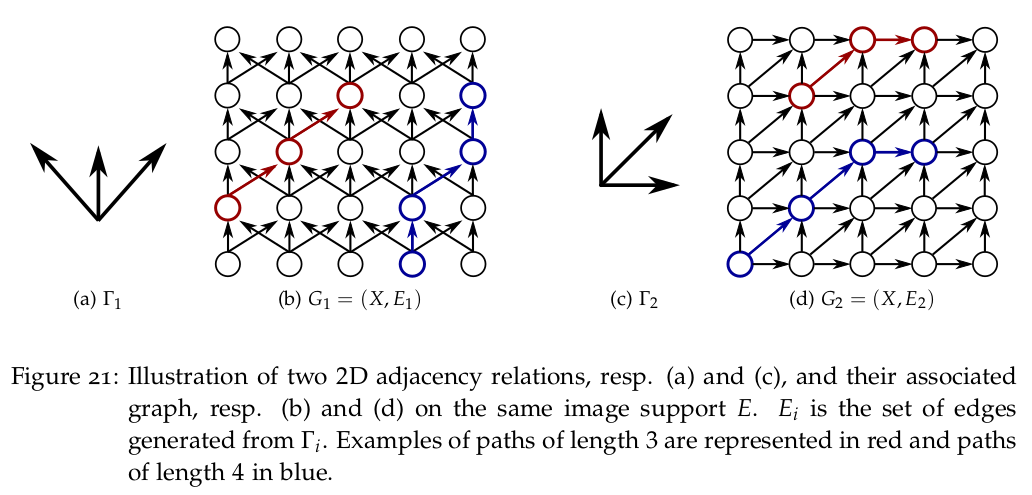
\includegraphics[height=4cm]{Images/rorpo_path.png}
  \caption{Illustration de relations d'adjacences permettant de définir les éléments structurants de RORPO. Les éléments structurants définis pour des orientations spécifiques capturent l'ensemble des potentielles variations des structures de l'image.}
  \label{fig:rorpo_adjacency}
\end{figure}

Les ouvertures sont calculées avec des éléments structurants définis dans 7 orientations principales de l'espace 3D de manière à capturer les objets de différentes formes tel que les blobs, les structures linéaires et les plateaux. Une étape finale consiste à classifier les différentes formes en triant les orientations des éléments structurants. En effet, pour des objets tubulaires, tous les éléments structurants sont orientés dans la même direction. RORPO est complétement lié à son espace d'échelle (Sec. \ref{sec:EA:rehaussement:echelle:granulometrie}), contrairement aux mesures de tubularité basé sur des valeurs propres qui peuvent s'adapter à plusieurs espaces (gaussien, flux, phase).

\section{Diffusion}
\label{sec:EA:rehaussement:diffusion}

Les méthodes de diffusion sont une classe à part dans le rehaussement des vaisseaux. L'objectif des cadres de diffusion est d'améliorer le signal des vaisseaux en homogénéisant leur intensité et en renforçant leurs bordures. Pour cela, les filtres de diffusion proposent un schéma de lissage itératif qui prend en compte la géométrie des structures à lisser.

HDCS \cite{Mendrik2009_HDCS} (Hybrid diffusion with continuous switch), propose un lissage hybride combinant lissage isotropique de régions et lissage basé sur les bordures. Ces deux lissages sont combinés avec une mesure de la géométrie locale afin d'appliquer une combinaison linéaire des deux filtres la plus adaptée.

VED \cite{Manniesing2006_VED} (Vessel enhancement diffusion) propose un lissage basé sur les méthodes de rehaussement hessiens. Ce cadre permet ainsi d'homogénéiser la réponse de n'importe quel filtre de rehaussement hessien en lissant selon le sens du rehaussement.

\begin{figure}[ht]
  \centering
  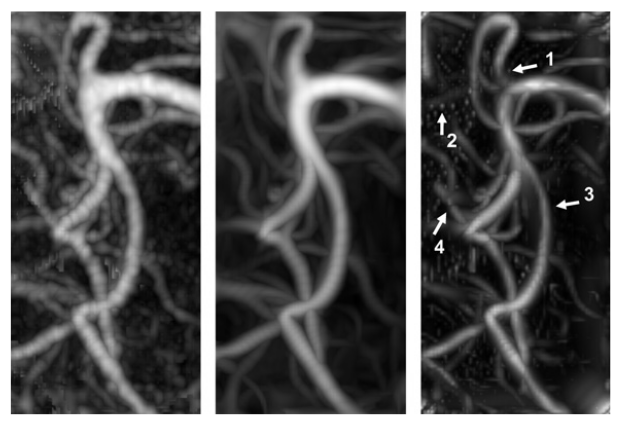
\includegraphics[height=4cm]{Images/VED.png}
  \caption{Comparaison de VED+Frangi (centre) contre Frangi (droite). Le rehaussement est lissé et l'homogénéité générale des vaisseaux est renforcé.}
  \label{fig:custom_fig}
\end{figure}

Ces méthodes itératives sont coûteuses en temps de calcul et nécessitent une paramétrisation supplémentaire pour contrôler la force du lissage ainsi que le nombre d'itérations nécessaire.

\section{Bilan et orientation des travaux}
\label{sec:EA:bilan}

Les constatations émises après l'état de l'art de la segmentation sont sensiblement les mêmes pour le rehaussement de vaisseaux. Les articles originaux testent souvent leurs méthodes sur des structures synthétiques simples ou des exemples variés. Elles sont toujours testées contre deux à quatres autres méthodes. Lorsqu'ils sont utilisés sur des données réelles, les filtres de rehaussement sont largement appliqués avec les paramètres recommandés par l'auteur, sans adaptation à une application particulière.

Quelques travaux portent sur la comparaison des filtres de rehaussement. Luu et al. \cite{Luu2015_liver_vesselness_comparison} proposent une comparaison de trois filtres de rehaussement et trois filtres de diffusion pour la tomodensitométrie du foie. Phellan et al. \cite{Phellan2017_Brain_vesselness_comparison} proposent une comparaison de six filtres de rehaussement et trois filtres de diffusions pour l'IRM du cerveau et un jeu de données synthétiques.

Cependant, ces travaux ne nous permettent pas de répondre à plusieurs questions :

\begin{itemize}
\item Quel filtre utiliser pour l'IRM du foie ?
\item Quel est l'impacte de la paramétrisation sur la réponse des filtres ?
\item Quels types de vaisseaux sont le mieux rehaussés ?
\item Quel est l'impacte des filtres de rehaussement indépendamment de la segmentation ?
\end{itemize}

Dans le chapitre suivant, nous proposons d'étudier la construction d'un banc de tests nous servant de support pour étudier ces problématiques. Celui-ci nous permettra ensuite d'effectuer une analyse poussée des filtres de rehaussement des vaisseaux sanguins dans les chapitres suivants.